%---------------------------------------------------------------
\chapter{Introduction}
%---------------------------------------------------------------
\setcounter{page}{1}

\section{Motivation, Focus of Thesis}

The theory of finite automata is an important part of the computer science curriculum at FIT CTU in Prague and other universities around the world. And although there is a lot of resources one can learn from, there is a lack of those that utilize modern tools. One of such modern tools is the iPad (and touch devices in general). This thesis will fill in this gap as the result will be a finite automata editor application for iPad.

Furthermore, I will expand on the recent work done at FIT CTU in Prague concerning the development of algorithms library and, more importantly for this thesis, finite automata algorithms including simulating input. This library is named \href{https://alt.fit.cvut.cz/}{Algorithms Library Toolkit} (ALT) \cite{alt} and it has been open sourced.

The main motivation of this thesis is to improve how students learn finite automata and more specifically, enhance the current course BI-AAG that is taught at FIT CTU in Prague. It is also an opportunity to use the ALT in practice and create a concrete example of how it can be leveraged.

\section{Thesis Goals}

The main goal of this thesis is to implement a prototype of an automata editor for iPad. This application should enable users to create and edit finite automata with emphasis on touch-based input.
I will also study the ALT's web interface \cite{state-maker} \cite{web-alt}, ALT itself focusing on design and drawing of finite automata, the possibilities of strokes detection on touch devices, and the approaches of shape detection, especially those used in automata drawing on iOS platform.

After the initial study of current approaches and theory, I will implement a prototype of a finite automata editor iPad app that will be capable of recognizing finite automaton elements from strokes and simulating input.

I will then conduct a usability testing to assess the usability and shortcomings of the prototype.

\section{Thesis Structure}

Let me now introduce you to the structure of the rest of the thesis:

\begin{itemize}
\item In \textbf{Chapter 2} I will go over the necessary theoretical background to properly explain terms and concepts on which it will be built upon later.

\item \textbf{Chapter 3} is concerned with the analysis of already existing solutions of creating an automata editor, the existing ALT web interface and ALT itself.

\item \textbf{Chapter 4} is about the design of the editor itself.

\item In \textbf{Chapter 5} I will write about the implementation.

\item \textbf{Chapter 6} will go into the specifics of usability testing and its outcomes.

\item \textbf{Conclusion} is the last chapter of this thesis where I will assess the success of fulfilling the aforementioned goals and lay out possible future development.

\end{itemize}

\chapter{Theory}
\label{chap:theory}

Firstly,  I will need to define terms and formal definitions concerning mainly finite automata theory, as that is the main subject of this thesis, and then machine learning as some of its concepts were important during the implementation. 

\section{Formal Languages and Grammars}
 
The following definitions are taken from Automata and Grammars by Eliška Šestáková \cite{automata-and-grammars}, Introduction to Automata Theory, Languages, and Computation \cite{introduction-automata}, and materials from BIE-AAG course \cite{lectures}.

\subsection{Formal Languages}

\begin{definition}
Alphabet (conventionally denoted by $\Sigma$) is a finite set whose elements are called symbols.
\end{definition}
Alphabets therefore can be:
\begin{itemize}
    \item $\Sigma$ = \{0, 1\}
    \item $\Sigma$ = \{a, b, c, d, e\}
    \item $\Sigma$ = \{one, two\}
\end{itemize}

\begin{definition}
String (word) over an alphabet is a finite sequence of symbols from that alphabet.
\end{definition}
\begin{itemize}
    \item $\epsilon$ - \textit{empty string} (string with zero occurences of symbols)
    \item $\Sigma^{*}$ - set of all strings over $\Sigma$
    \item $\Sigma^{+}$ - set of all nonempty strings over $\Sigma$
\end{itemize}
For a binary alphabet $\Sigma$ = \{0, 1\} $\epsilon$, 1001, 100, 1, 001 are all strings over the alphabet $\Sigma$.

\begin{definition}
Formal language L over an alphabet $\Sigma$ is any subset of all the strings over $\Sigma$ - i.e., $L \subseteq \Sigma$
\end{definition}
For a binary alphabet $\Sigma$ = \{0, 1\} a formal language over $\Sigma$ is then subsets of \textit{all} binary strings. We can denote the language either by:
\begin{itemize}
    \item enumeration notation where all possible strings in the language are listed, e.g.: $\textit{L}_1 = \{\epsilon\}, \textit{L}_2 = \{1\}, \textit{L}_3 = \{0, 00, 000, 01\}$.
    \item set-builder notation where the languages are described in the following way: \{ w $\mid$ something about w \}. Examples are: $\textit{L}_4 = \{\textit{w} \mid \textit{w} \in {0,1}^* \wedge \left\lvert \textit{w} \right\rvert \mod 2 = 0\}$, $\textit{L}_5 = \{0^\textit{n}1^\textit{n} : \textit{n} \in \mathbb{N}_0\}$.
\end{itemize}

\subsection{Grammar}

Grammars are used to generate languages. You can find how they are defined below:

\begin{definition}
    \textit{Grammar} is a quadruple of G = (N, $\Sigma$, P, S) where:
\end{definition}
\begin{itemize}
    \item \textit{N} is a finite non-empty set of nonterminal symbols.
    \item $\Sigma$ is a finite set of terminal symbols ($\Sigma$ $\cap$ \textit{N} = $\emptyset$). Note that \textit{N} $\cap$ $\Sigma$ = $\emptyset$.
    \item \textit{P} is a finite set of \textit{production rules}, assuming the following form:\\

    \centerline{$\alpha\textit{A}\beta \rightarrow \gamma$ ($\alpha, \beta, \gamma \in (\textit{N} \cup \Sigma)^*$)}
\end{itemize}

The following is an example of a grammar that describes the language \textit{L} = $\{01^\textit{n}0 : \textit{n} \in \mathbb{N}_0\}$:
Grammar \textit{G} = (\{\textit{A}, \textit{S}\}, \{0, 1\}, \textit{P}, \textit{S}) where \textit{P}:
\begin{itemize}
    \item \textit{S} $\rightarrow$ 0\textit{A}
    \item \textit{A} $\rightarrow$ 1\textit{A}
    \item \textit{A} $\rightarrow$ 0
\end{itemize}

\subsection{Chomsky Classification of Grammars}

Grammars are divided into four classes where they differ in their production rules. 

\begin{definition}
    Let G = (N, $\Sigma$, P, S). We say that G is:
\end{definition}
\begin{enumerate}
    \item \textit{Unrestricted grammar} (type 0), if every rule is in the form of:
    
    \centerline{$\alpha\textit{A}\beta \rightarrow \gamma$ ($\alpha, \beta, \gamma \in (\textit{N} \cup \Sigma)^*$, $\textit{A} \in \textit{N}$)}
    \item \textit{Context-sensitive} (type 1), if every rule is in the form of:

    \centerline{$\gamma\textit{A}\delta \rightarrow \gamma\alpha\delta$ ($\gamma, \delta \in (\textit{N} \cup \Sigma)^*$, $\textit{A} \in \textit{N}$, $\alpha \in (\textit{N} \cup \Sigma)^+$)}
    or in the form of $\textit{S} \rightarrow \epsilon$ if \textit{S} is not present on the right hand side of any rule of a given grammar.
    \item \textit{Context-free grammar} (type 2) if every rule is in the form of:

    \centerline{$\textit{A} \rightarrow \alpha$ $(\textit{A} \in \textit{N}, \alpha \in (N \cup \Sigma)^*)$}
    \item \textit{Regular grammar} (type 3), if every rule is in the form of:

    \centerline{$\textit{A} \rightarrow \textit{a}$ or $\textit{A} \rightarrow \textit{aB}$ $(\textit{a} \in \Sigma, \textit{A}, \textit{B} \in \textit{N})$}
    or in the form of $\textit{S} \rightarrow \epsilon$ if \textit{S} is not present on the right hand side of any rule of a given grammar.
\end{enumerate}

\subsection{Classification of Languages}
Classification of languages, also known as the Chomsky hierarchy, has the following definition:
\begin{definition}
    We say that language is:
\end{definition}
\begin{enumerate}
    \item \textit{formal} if it is a formal language but is neither regular, context-free, context-sensitive, nor recursive enumerable. These languages are not accepted by a Turing machine.
    \item \textit{recursively enumerable} if and only if $\exists$ unrestricted grammar which generates it
    \begin{itemize}
        \item accepted by a Turing machine
    \end{itemize}
    \item \textit{context-sensitive} if and only if $\exists$ context-sensitive grammar which generates it
    \begin{itemize}
        \item recognized by a linear bounded Turing machine
    \end{itemize}
    \item \textit{context-free} if and only if $\exists$ context-free grammar which generates it
    \begin{itemize}
        \item recognized by a nondeterministic pushdown automaton
    \end{itemize}
    \item \textit{regular} if and only if $\exists$ regular grammar that generates it
    \begin{itemize}
        \item recognized by a finite automaton
    \end{itemize}
\end{enumerate}

For most of the thesis, only regular languages will be needed since those are recognized by finite automata. Finite automata will be defined in the following section.

\section{Finite Automata}

The final editor app will be for finite automata, therefore they are very important for this thesis. Informally, a finite automaton is a model for simple computation. States, that serve as memory, and transitions together form a \textit{control unit}. Along with a control unit, the finite automaton has a \textit{read-only input tape}, which is divided into individual cells, and the \textit{head} that scans the input tape as the automaton continuously reads it, cell by cell. Automaton starts in its initial state and with a head pointing at the first cell. As the input is read, the head moves until it has read all of the input tape. If there is a missing transition for an input, the automaton does not accept the input. Otherwise, it accepts the input if it is in a final state at the end of the input.

Let's define a finite automaton formally:
\begin{definition}
    Finite automaton is a quintuple \textit{M} = (\textit{Q}, $\Sigma$, $\delta$, $\textit{q}_0$, \textit{F}) where:
    \begin{itemize}
        \item \textit{Q} is a finite non-empty set of states
        \item $\Sigma$ is a finite input alphabet
        \item $\delta$ is the transition function (the exact definition is determined by which type of a finite automaton it is - see below)
        \item $\textit{q}_0 \in \textit{Q}$ is the initial state
        \item $\textit{F} \subseteq \textit{Q}$ is the set of initial states
    \end{itemize}
\end{definition}

Finite automaton can also be either a \textit{deterministic} finite automaton or a \textit{nondeterministic} finite automaton. This dictates the exact definition of $\delta$ - transition function.
For a deterministic finite automaton (DFA) the definition of $\delta$ is:\\
\centerline{$\delta$ is a mapping from \textit{Q} $\times$ $\Sigma$ to \textit{Q}}
$\delta$ for a nondeterministic finite automaton (NFA) is defined as:\\
\centerline{$\delta$ is a mappping from \textit{Q} $\times$ $\Sigma$ into the set of all subsets \textit{Q} (denoted by $2^\textit{Q}$)}
Expanding upon the difference between the definitions of the transition function:
\begin{itemize}
    \item DFA can only transition from one state to another, e.g. from $\textit{q}_2$ to $\textit{q}_3$ ($\textit{q}_2$, $\textit{q}_3$ $\in$ \textit{Q})
    \item NFA can transition to a set of states, e.g. from $\textit{q}_1$ to $\textit{q}_1$, $\textit{q}_2$ ($\textit{q}_1$, $\textit{q}_2$ $\in$ \textit{Q})
\end{itemize}
If we change the definition of NFA's $\delta$ to a mapping from \textit{Q} $\times$ ($\Sigma \cup \{\epsilon\}$) we allow, what are called, $\epsilon$-transitions that allow us to move to a different state while not reading any input from the tape. This finite automaton is then called a \textit{nondeterministic finite automaton with $\epsilon$-transitions}.

\subsection{Representation of Finite Automata}

Finite automata's transition functions $\delta$ are generally represented in the form of:
\begin{itemize}
    \item \textit{Formal notation}\\
    (NFA) $\delta$(\textit{S}, 0) = \{\textit{S}, \textit{A}\} (transition from the state \textit{S} and symbol 0 to the states \textit{S} and \textit{A})\\
    (DFA) $\delta$(\textit{A}, 0) = \textit{B} (transition from the state \textit{A} and symbol 0 to a single state, not a set of states, \textit{B})
    \item \textit{Weighted directed graph} (state diagram)\\
    Automata can be represented graphically as directed weighted graphs. Each state is represented as a vertice in the graph and final states are recognized by being a double circle, instead of a single one. Initial state is the one with an arrow that points to the state but does not start anywhere - it is often additionaly denoted with \textit{start}. The transitions are then directed edges between states. You can see a FA represented as a weighted directed graph in \ref{graph-representation}.
    \item \textit{Table}\\
    Table representation has in the first column all states where the initial state is marked with $\rightarrow$ while final states are marked with $\leftarrow$. In the first row, excluding the first column, there are symbols of the alphabet, $\Sigma$. In the rest of the rows are states (or a set of states) that will be transitioned to on a given input (defined in the first row). You can see an example of it in \ref{table-representation}.
\end{itemize}
\begin{figure}
\begin{tikzpicture}
    \node[state, initial] (q1) {$q_1$};
    \node[state, accepting, right of=q1] (q2) {$q_2$};
    \node[state, right of=q2] (q3) {$q_3$};
    \draw   (q1) edge[loop above] node{0, 1} (q1)
            (q1) edge[above] node{1} (q2)
            (q2) edge[bend left, above] node{0} (q3)
            (q3) edge[bend left, below] node{1} (q2);
\end{tikzpicture}
\caption{FA graph representation}\label{graph-representation}
\end{figure}
\begin{figure}
\begin{tabular}{||c|c|c||} 
    \hline
    $\delta_{NFA}$ & 0 & 1 \\ [0.5ex] 
    \hline\hline
    $\rightarrow \textit{q}_1$ & $\textit{q}_1$ & $\textit{q}_1$, $\textit{q}_2$ \\ 
    \hline
    $\leftarrow \textit{q}_2$ & $\textit{q}_3$ & \\
    \hline
    $\textit{q}_3$ &  & $\textit{q}_2$ \\
    \hline
\end{tabular}
\caption{FA table representation}\label{table-representation}
\end{figure}
In this thesis we will mostly be working with the representation in the form of a weighted directed graph as that is what will the users edit in the app.
This also concludes the theory about finite automata and formal languages.

\section{Machine Learning}

Machine learning does not have an exact definition but e.g. in the book Foundations of Machine Learning it's loosely defined as "computational methods using experience to improve performance or to make accurate predictions" \cite{ml-foundations}. \textit{Experience} means something we know from the past that we can leverage for making predictions in the future. Usually, this experience comes in the form of data. The book Foundations of Machine Learning \cite{ml-foundations} and materials from BIE-VZD from FIT CTU in Prague \cite{vzd-lectures} will be used further in this section to define terms and concepts necessary for this thesis.

\subsection{Classification}

Machine learning, in order to cluster problems that can be solved in a similar way, can be categorized into a few learning scenarios, most notably supervised and unsupervised learning. The learning scenario is a basic description of what type of data we have, how we receive the data and the test data that we use to evaluate the learning algorithm.

\begin{itemize}
    \item \textit{supervised learning}: Our goal is to explain \textit{variable Y} given \textit{independent variables} $\textit{X}_0$, $\textit{X}_1$, ..., $\textit{X}_{\textit{p} - 1}$. We do this by finding a "function" for which most of its examples the following holds:\\
    \centerline{\textit{Y} $\approx$ \textit{f}($\textit{X}_0$, $\textit{X}_1$, ..., $\textit{X}_{\textit{p} - 1}$)}
    \item \textit{unsupervised learning}: Our goal is to find structures of "similar" data. We do not predict any class and there is no clear way to assess the quality of an unsupervised learning algorithm since it is not clearly defined what the end result should be.
\end{itemize}

In this thesis we will be only interested in supervised learning. We can also divide common problems that machine learning is trying to solve by learning tasks - that includes classification, regression, ranking, clustering, etc. Let's look more closely at classification which will be later used in the implementation:
\begin{itemize}
    \item Classification is a problem of assigning a category to each item.
\end{itemize}
It is also a problem solved via supervised learning. To expand on the definition of supervised learning from above, classification is a special case where \textit{Y} has only a few (countable amount) of values. The simplest example of classification is \textit{binary classification}. E.g. we want to predict whether a patient has flu and our data - gender of a patient, whether a person can leave the bed, etc. - can be represented in a binary format (yes/no).

\chapter{Analysis}
\label{chap:analysis}

In the analysis I will study the following:
\begin{itemize}
    \item existing applications that enable users to edit finite automata, including ALT web interface
    \item ALT itself, focusing on design and drawing of finite automata
    \item possibilities of detection of strokes on touch devices.
\end{itemize}

\section{Existing Applications}

This section will be concerned with the study of existing applications - be it applications for mobile or web.

\subsection{ALT Web Interface}

ALT web interface has been built as a part of a bachelor's thesis made by Michael Vrána \cite{web-alt} leveraging work already done in ALT itself. ALT web interface uses Pipe-and-Filter \cite{pipe-and-filter} architecture to easily combine input and outputs of the individual algorithms that ALT offers which can be seen in figure \ref{alt-web-interface-screen}. Apart from ALT algorithms it also includes a finite automata editor done by Petr Svoboda \cite{state-maker}.

\begin{figure}
    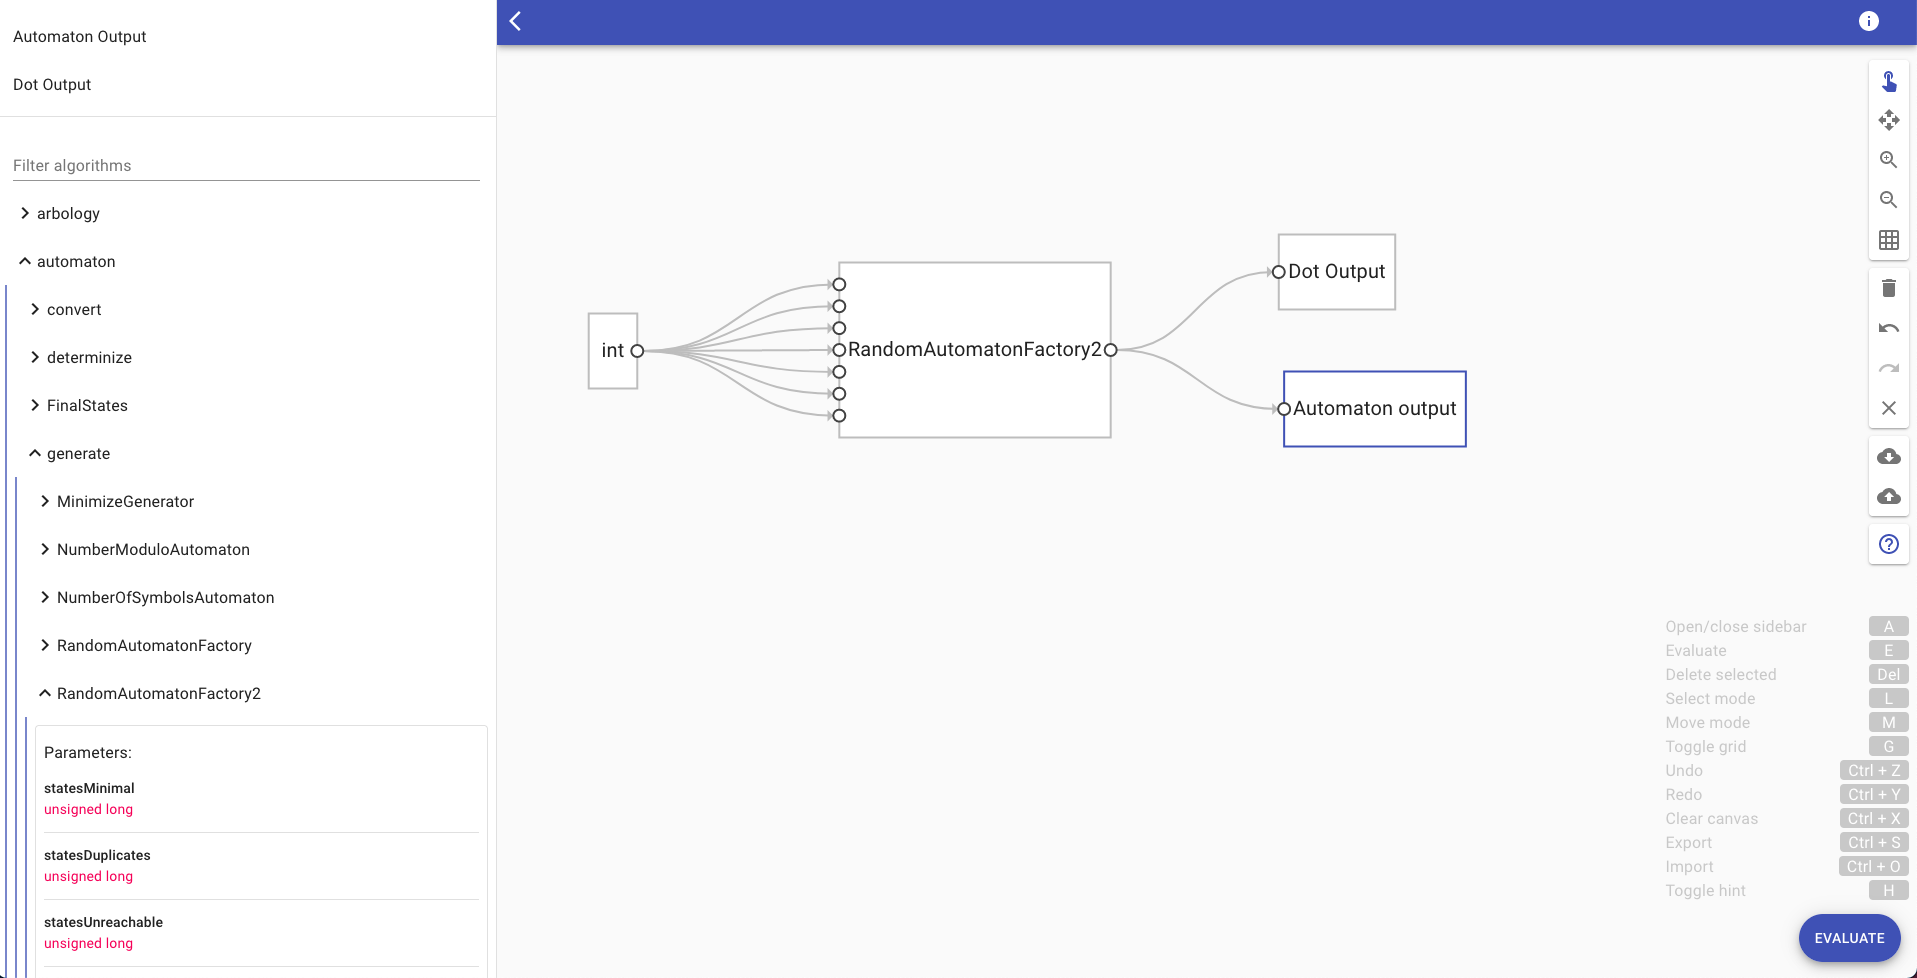
\includegraphics[width=\textwidth]{alt-web-interface}
    \caption{ALT web interface screenshot}\label{alt-web-interface-screen}
\end{figure}

This finite automata editor is called Statemaker and you can see a screenshot of how it looks in figure \ref{statemaker-screen}. To summarize its capabilities, users can:
\begin{itemize}
    \item Add states.
    \item Add transitions between states.
    \item Edit transition string.
    \item Mark states as initial or final.
    \item Remove states and transitions.
    \item Import and export automaton in supported formats.
    \item Automatic positioning of transitions and states.
\end{itemize}
All of the above features work reliably and are done in an intuitive manner - a user can quickly understand how to work with all the components. The most notable missing feature is the easy simulation of input - this can be done via the ALT web interface but if someone is looking for only editing FAs and simulating whether the input string is accepted, they have to transition between two interfaces. The benefit is that they can then tap into all the other functionality that ALT offers. The author of Statemaker has chosen React and Typescript as underlying technologies \cite{state-maker}.

\begin{figure}
    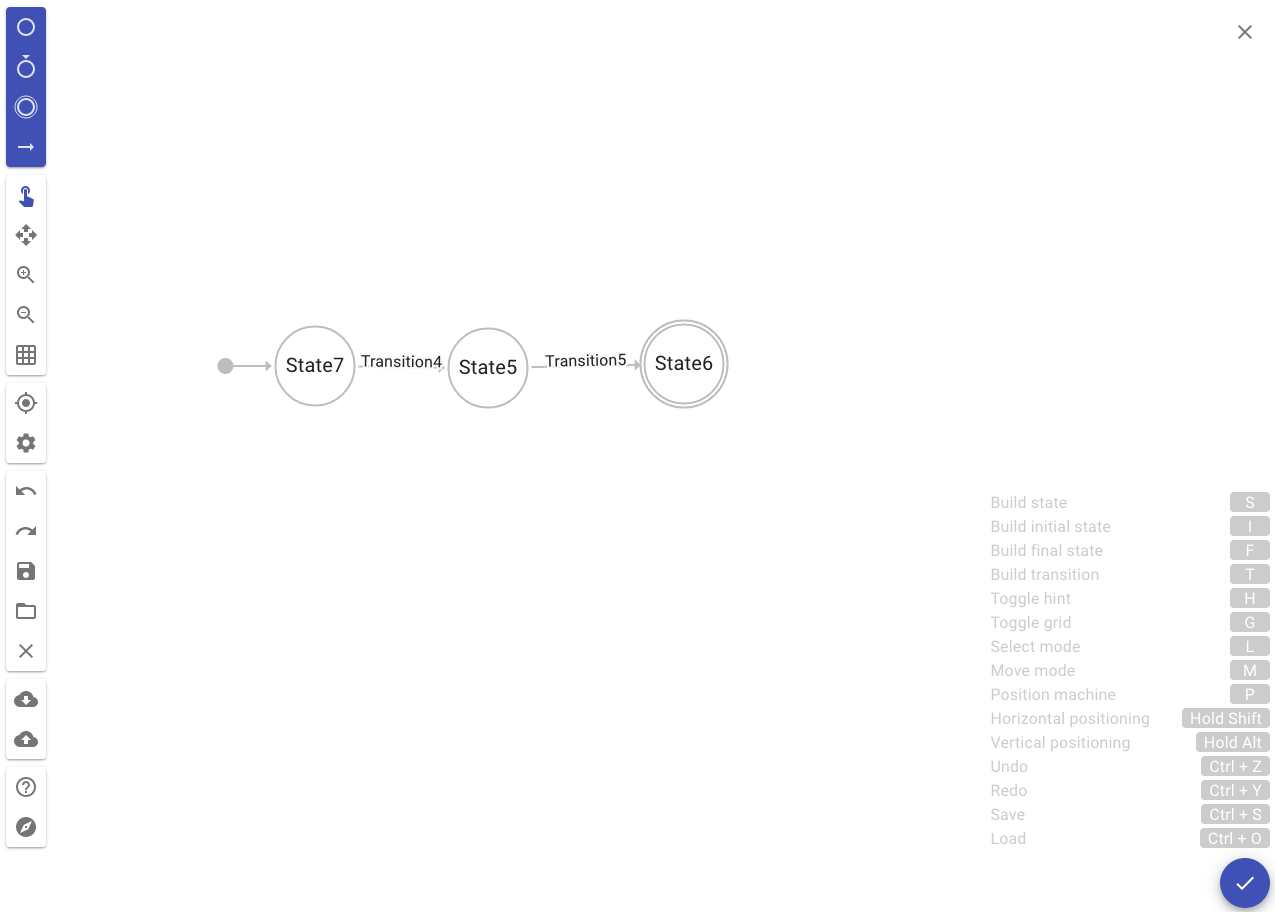
\includegraphics[width=\textwidth]{statemaker}
    \caption{Statemaker screenshot}\label{statemaker-screen}
\end{figure}

\subsection{Other Existing Applications}

As the main goal of this thesis is to write a finite automata editor for iPad, in this part I will study existing applications mainly for touch devices. 

One of such applications is TuringSim \cite{turingsim}. Although it is not for FAs but a Turing machine, it also consists of an editor where the user can add and edit states and transitions, thus making it similar to a FA editor. You can see its interface in figure \ref{turingsim-screen}. This editor lets users add and edit automaton's states and transitions. Users can also simulate input on the Turing machine's read-and-write tape. Editing of the automaton is done only via tap gestures which is similar to Statemaker with the difference that there are no distinct buttons for those actions. Therefore, it does not fully utilize the potential of touch devices as the UX is very similar to what would one experience on the web. Unfortunately, the app on the iPad is broken at the moment as it is missing a bottom toolbar for simulating input.

Finite Automata \cite{finite-automata-app} is another iPad app. In this app user can not edit automata in their weighted graph representation but instead has to use a command line that takes individual commands which are described in the app. This app does not utilize touch device features at all.

There are also apps available as desktop applications. One is a Finite Automaton Editor by Jaime Rangel-Mondragon that is available as an interactive Wolfram notebook \cite{wolfram-editor}. This app allows you to edit the automaton via a transition table and does not allow to simulate any input. Automata Editor by Max Shawabkeh \cite{automata-editor-max} is another desktop application. In it users can create and edit their automaton either via a table representation or a regular expression. There are also features such as NFA determinization, simulating input, and minimizing DFA. Thus, it has a powerful feature set but one has to be already familiar with the FA theory to be able to utilize it fully. It should also be noted that the feature set is a subset of what the ALT web interface offers.

\begin{figure}
    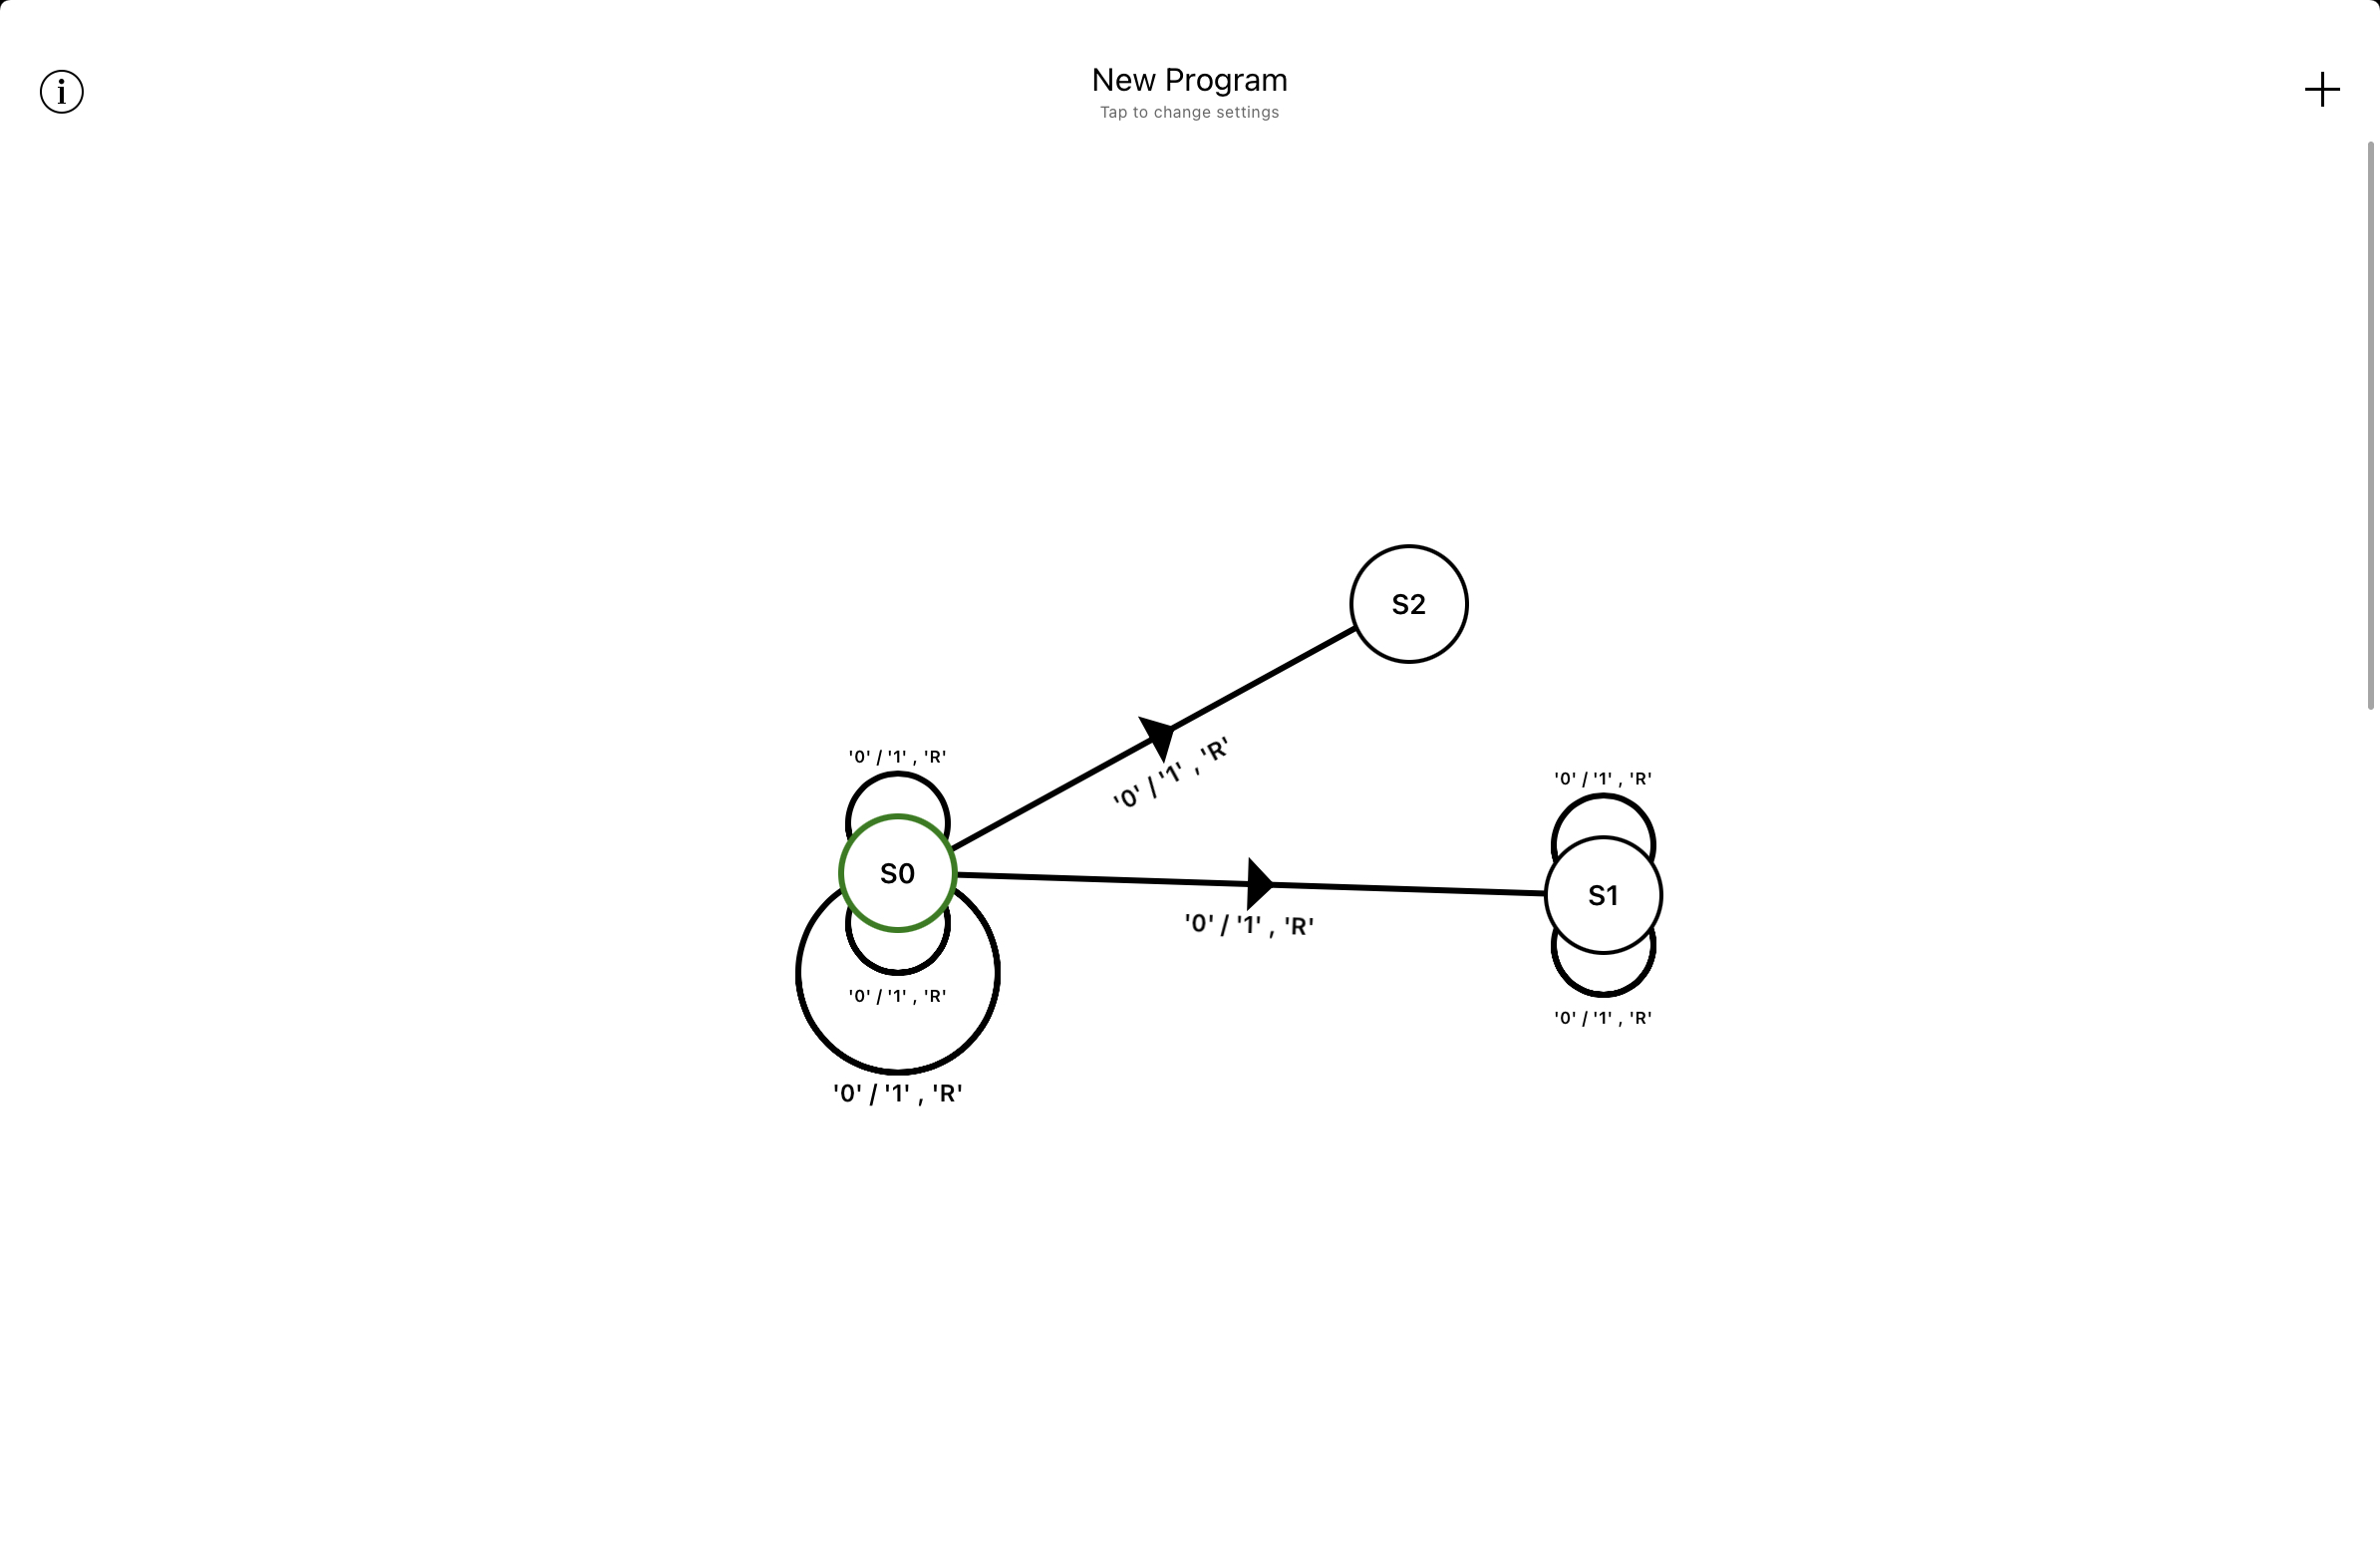
\includegraphics[width=\textwidth]{turingsim}
    \caption{TuringSim interface screenshot}\label{turingsim-screen}
\end{figure}

\section{ALT}

I will now go over ALT and its features that can be leveraged for simulating FA input. The code of ALT is available on GitLab \cite{gitlab} where there are multiple repositories in the group Algorithms Library Toolkit (webui-client, infrastructure, etc.) - that includes a repository Algorithms Library Toolkit Core \cite{alt-code}, a library written in C++ \cite{c++}. There we can find algorithms that can later be used for a FA editor. The code is divided into multiple modules that are then built and linked together using CMake \cite{cmake}. The most important modules for this thesis are \textit{alib2data} and \textit{alib2algo} where alib2data contains FA models and alib2algo algorithms for simulating input.

\subsection{FA Model}

Multiple FA types are supported by ALT - which includes a deterministic and a nondeterministic finite automaton, as well as a nondeterministic finite automaton with $\epsilon$-transitions. There is also extended NFA that has regular expressions as its transitions. These models serve as a description of an automaton - its states, transitions, etc. To create e.g. NFA with $\epsilon$-transitions one can use its constructor where it is possible to specify its states and input alphabet. For adding transitions there is a method called \lstinline{addTransition}. Both can be seen in figure \ref{epsilon-nfa-methods}.

\begin{lstlisting}[language=C++, caption=EpsilonNFA example methods, label=epsilon-nfa-methods]
// Creates a new instance of the Automaton
// with a concrete initial state.
explicit EpsilonNFA ( 
    ext::set < StateType > states,
    ext::set < SymbolType > inputAlphabet, 
    StateType initialState, 
    ext::set < StateType > finalStates
);
// Add a transition to the automaton.
bool addTransition ( 
    StateType from,
    common::symbol_or_epsilon < SymbolType > input,
    StateType to 
);
\end{lstlisting}

\subsection{FA Algorithms}

ALT offers a multitude of algorithms that can be run on finite automata - such as minimization, determinization, and simulating input. Simulating input can be found in \lstinline{Accept.h}, \lstinline{Result.h}, \lstinline{Occurrences.h}, and \lstinline{Run.h} that contain classes of the same name. \lstinline{Accept} has a method called \lstinline{accept} that returns a simple boolean indicating whether the input has been accepted or rejected. \lstinline{Result}'s \lstinline{result} method returns a state where the simulation ended and \lstinline{Occurrences}'s \lstinline{occurences} method returns a set of indices where the automaton has passed a final state. \lstinline{Run}'s returned value is then a combination of \lstinline{Accept} , \lstinline{Result} and \lstinline{Occurences} where it contains the combined output of all those classes. The \lstinline{Run}'s function \lstinline{calculateStates} can be seen in \ref{calculate-states}.

\begin{lstlisting}[language=C++, caption=Run's calcuteStates function, label=calculate-states]
template < class SymbolType, class StateType >
static ext::tuple < 
    bool, 
    ext::set < StateType >, 
    ext::set < unsigned > 
> calculateStates ( 
    const automaton::EpsilonNFA < 
        SymbolType, 
        StateType 
    > & automaton, 
    const string::LinearString < SymbolType > & string
);
\end{lstlisting}

\section{Strokes Recognition}

The final prototype will include recognizing automaton elements from drawing. In this section I will go over available methods of how to achieve it.

\subsection{Google ML Kit}

Google offers a framework called ML Kit that includes what they call "Digital Ink Recognition". This lets you construct a stroke from points drawn on the screen and create an \lstinline{Ink} object from those strokes. It also includes base models for recognizing text and even some basic shapes like arrow and rectangle. If you want to create your own model with TensorFlow Lite \cite{tensorflow}, you are forced to use "Image Labeling". Since the editor should support creating cycles, it is necessary to create a custom model because that shape is not supported by any of the base models for Digital Ink Recognition.

\subsection{Core ML}

Apple's CoreML framework supports a variety of use cases - analysis of images, processing text, converting audio to text, and identifying sounds in audio \cite{coreml}. It does not, however, support anything like Digital Ink Recognition - but for the editor it is suitable to use analysis of images because it is possible to create an image from the screen and pass that to the model. Apple also provides some models already in CoreML format \cite{coreml-models} but not any of them are applicable for the FA editor's use case. Therefore, a custom model for CoreML would be necessary as well.

Considering that CoreML is bundled in the system and Google ML Kit needs to be installed separately, increasing the app's size and incurring the maintenance burden, I have opted for CoreML. This decision has also been made based on the fact that both frameworks do support TensorFlow, although, for CoreML it needs to be first converted to its format.

\subsection{Creating the CoreML Model}

There are multiple ways how to create a CoreML model, though, they generally fall into two categories:
\begin{itemize}
    \item ML model created by ML libraries that are not from Apple such as TensorFlow or Keras \cite{keras} and then converted with coremltools \cite{coremltools} to the CoreML format.
    \item ML model created by framework or application that outputs CoreML directly.
\end{itemize}

For creating CoreML models directly there is either Create ML \cite{create-ml} or turicreate \cite{turicreate}. Create ML, at the time of writing, supports only image classification, whereas turicreate has built-in support for drawing classification. Although both image classification and drawing classification operate on images, the important distinction is that drawing classification takes 28x28 grayscale bitmap as input. The drawing classification is also tailored for inputs created by Apple Pencil \cite{drawing-classification}, thus I have chosen to use it instead of libraries such as TensorFlow. It should be noted, though, that turicreate leverages TensorFlow as a lower-level framework and it should serve to streamline the development of CoreML models.

\chapter{Automata Editor Design}
\label{chap:design}

In this chapter I will go over some decisions made, such as which technology I have decided to use, and over the design of the editor - how the app will look and how users will interact with the editor.

\section{Touch Device}
The main reason why this prototype is meant for a touch device is to simulate as much as possible the experience of drawing FAs on regular paper. There were three main options possible:
\begin{itemize}
    \item create a touch-friendly web interface
    \item implement an app for Android
    \item target iPad devices
\end{itemize}
Creating a touch-friendly web interface would have the benefit of being universal and not tied to a specific platform. But native apps offer better precision and developers can tap into OS APIs that are tailored for touch. The choice between Android and iPad was less clear but iPad has the benefit of Apple Pencil \cite{apple-pencil} that offers high precision that will make the user experience better.

\section{Used Technologies}

I will now cover which technologies are used in the app and why I have chosen them. A lot of decisions have been influenced by focusing on the iPad and, even more specifically, by targeting iPad devices along with the Apple Pencil. 

\subsection{Language}

Choosing a language in which one will write the application is an important first step. For iOS applications I could have generally used:
\begin{itemize}
    \item Objective-C
    \item Swift
    \item cross-platform framework
\end{itemize}

Objective-C was designed by Brad J. Cox at the start of the 1980s and was then licensed by NeXT Software in 1988. Then in 1996 NeXT Software was acquired by Apple - along with Objective-C. Apple has then chosen Objective-C as the main language for OS X and in 2007 for the new operating system iOS \cite{objective-c-programming}. On the Apple developer website it is described as "superset of the C programming language and provides object-oriented capabilities and a dynamic runtime" \cite{objective-c}. Objective-C has been thus the main programming language for years. Nowadays, Objective-C is not anymore that popular and ranks 23rd in the language popularity as per TIOBE index \cite{tiobe-index}. Apple has rather shifted their focus to Swift and some of the new frameworks, like SwiftUI \cite{swiftui}, are only available in Swift. Swift is therefore a much better option if one is starting a new iOS app.

Using a cross-platform framework - such as React Native \cite{react-native} or Flutter \cite{flutter} that are written in Javascript and Dart, respectively - was also a possibility. But to leverage the Apple Pencil fully it was necessary to use PencilKit \cite{pencilkit} and for interacting with that framework one would have to write native code. Thus, I have decided to use Swift as the main language.

\subsection{UI Framework}

At the time of writing it is possible to use two UI frameworks offered by Apple to write UI code. Those are UIKit \cite{uikit} or, already mentioned, SwiftUI \cite{swiftui}. SwiftUI is a newer framework than UIKit, released in 2019 \cite{swiftui-release}. In the Thinking in SwiftUI book it is described as a "radical departure from UIKit, AppKit, and other object-oriented UI frameworks" \cite{thinking-in-swiftui}. SwiftUI offers a more declarative approach, quite similar to React \cite{react} used in the web development. Declarative UIs have the benefit of less code since it enables the framework to do more on behalf of the developer. This comes at a cost of lesser control. Getting back to SwiftUI, specifically, one of its major drawbacks is that not all components, that are written in UIKit, are available in SwiftUI. But there is very strong support for SwiftUI-UIKit interoperability \cite{swiftui-interop} and thus it is always possible to use UIKit when necessary. The fact that SwiftUI offers faster development due to its declarative nature and SwiftUI previews \cite{swiftui-preview} has made it a better candidate than UIKit, especially for a prototype. Therefore, I have decided to use SwiftUI as the main UI framework.

\subsection{PencilKit}

I have already mentioned the PencilKit framework but it is not the only way how to let users draw with either their finger or Apple Pencil. One can also use CGContext which is a "Quartz 2D drawing environment" \cite{cgcontext}. For drawing in CGContext it is necessary to observe user's touches and draw a path based on those touches. CoreGraphics framework, which CGContext is a part of, does not bundle any component that would handle the drawing for the developer \cite{coregraphics}. PencilKit, however, has a component called \lstinline{PKCanvasView} \cite{pkcanvasview}. By using this component, the PencilKit framework handles for us how to draw strokes made by the user. \lstinline{PKCanvasViewDelegate} enables listening to changes of the drawing. The \lstinline{drawing} property of type \lstinline{PKDrawing} then allows for programmatic modifications of the drawing - which will be used to render the FA elements after they are recognized.

For the purposes of the prototype, PencilKit is a better fit because it offers more by default while still allowing for minor modifications. If some more custom behavior of e.g. rendering strokes was needed, though, it would be necessary to use the CoreGraphics framework. To make a possible migration between those frameworks as seamless as possible, the PencilKit framework should be well-contained.

\subsection{Architecture}

There is no recommended architecture by Apple for apps written on top of SwiftUI frameworks. It is also entirely possible to create an app without adhering to any architecture. This code, though, is then more difficult to maintain for a longer period.

One possible architecture is MVVM \cite{mvvm}. A diagram of this architecture can be seen in figure \ref{mvvm}. It enables developers to have a clear boundary between UI code and business logic and is a good option for either UIKit or SwiftUI applications. One of its drawbacks is that it can sometimes lead to imperative code where developers call a function and act based on its inputs. The alternatives are (among others) architectures inspired by Redux. A diagram of Redux is depicted in figure \ref{redux}. The main difference between Redux and MVVM is that MVVM is event-driven, whereas Redux is data-driven. The data-driven approach is much more closer to declarative programming since the state of the application describes how it should look. Thus I have decided that Redux-like architecture will be a better option.

One of concrete implementations of Redux architecture is the Composable Architecture by Point-Free \cite{tca}. This architecture is based on Redux but it has some modifications such as handling of side effects. It also makes testing more exhaustive by asserting that no action that you do not expect is run, as well as that the state is not changed in any other way than you describe in your test. Considering all of the above, I have chosen to use the Composable Architecture. 

\begin{figure}
    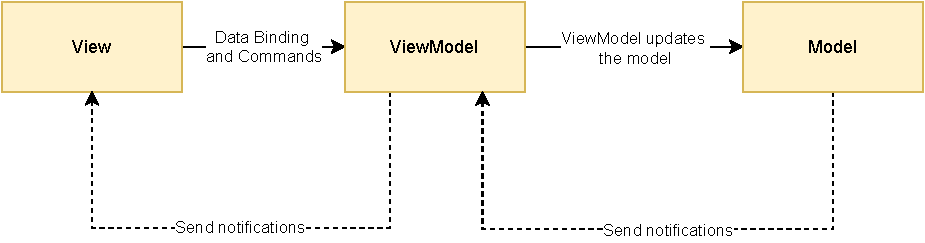
\includegraphics[width=\textwidth]{MVVM}
    \caption{MVVM architecture diagram \cite{mvvm}}\label{mvvm}
\end{figure}

\begin{figure}
    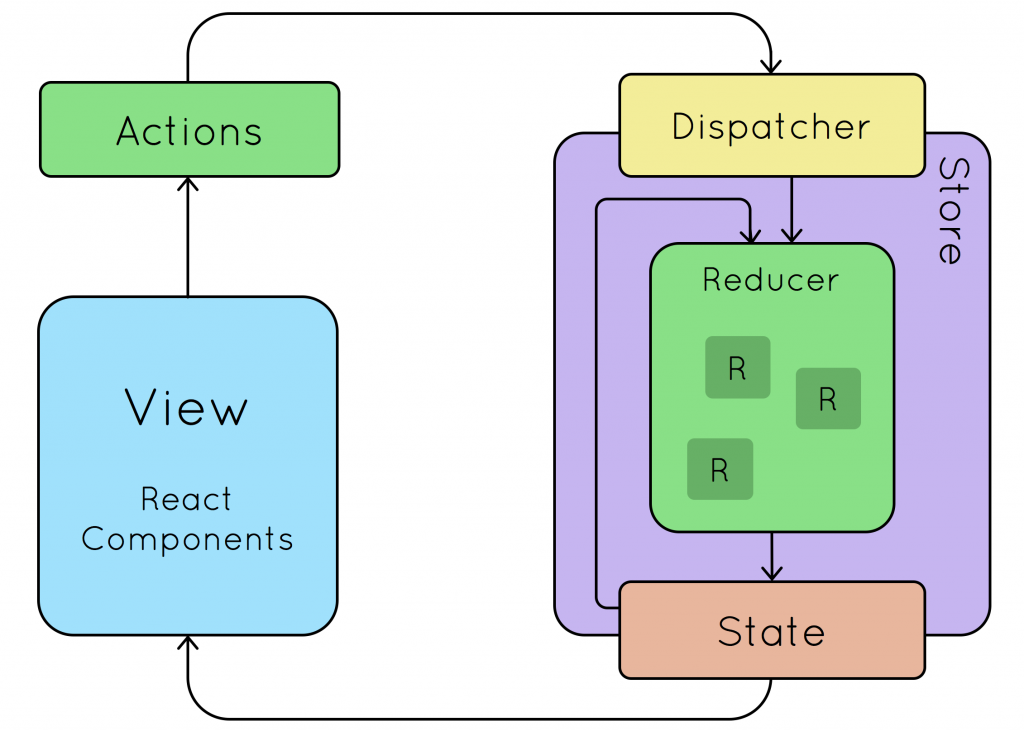
\includegraphics[width=\textwidth]{redux}
    \caption{Redux architecture diagram \cite{react-redux}}\label{redux}
\end{figure}

\section{ALT Integration}

I have already talked about ALT in chapter \ref{chap:analysis}. I have not discussed there, however, how ALT will be integrated into the application. That is now possible as I have stated that the app will be written in Swift. As already mentioned, ALT is a library written in C++. There exists a Swift-C++ interoperability manifesto \cite{swift-c++-manifesto} but this manifesto only goes over what it would take to make C++ and Swift interoperable but not even all functionalities of C++ have their discussions of how they could be ported to Swift. However, there is well-supported interoperability between Swift and Objective-C \cite{swift-objc-interoperability}. For Objective-C and C++, interoperability is supported via a language iteration of Objective-C called Objective-C++. It is even e.g. possible to "include pointers to Objective-C objects as data members of C++ classes" \cite{objc++}. I first tried to integrate ALT directly and compile it right via Xcode. Since ALT is built via CMake \cite{cmake} and does not have a simple setup, I then resorted to pre-building the necessary modules and afterwards bundling them in the application. I will go over the details in chapter \ref{chap:implementation}.

\section{User Interface}

As a final section of this chapter, I will discuss the design of the UI. The design has been heavily influenced by the fact that one of the main goals was to imitate the experience of drawing FAs on a piece of regular paper. The app should let users to:
\begin{itemize}
    \item create FA states, transitions, and cycles
    \item delete and rearrange all of the above
    \item name states
    \item specify symbols for transitions
    \item simulate input and see whether the input was or was not accepted by the automaton
\end{itemize}

\subsection{Canvas}

Canvas is the most important part of the editor since it is the space where users can draw FA elements. After each stroke, a function will be run that will evaluate the stroke to determine which FA state the user has drawn. The flow of recognizing the FA elements is graphically represented in figure \ref{app-flow}. The app first waits for the user to make a stroke, after a stroke is made its representation is sent to the ML model which recognizes the type of FA element, a state is updated with the new element and it is drawn on the canvas. Then the app again waits for another stroke.

\begin{figure}
    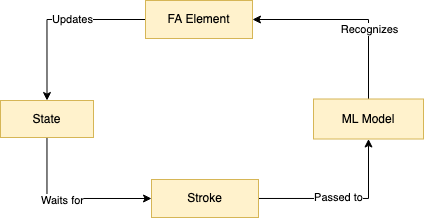
\includegraphics[width=\textwidth]{app-flow}
    \caption{Flow of recognizing FA elements from strokes}\label{app-flow}
\end{figure}

\subsection{State}

The app needs to be able to work with three FA elements - state, transitions and a cycle (a special case of transition that starts and ends in the same state). These elements should be represented the same way as they are in the weighted directed graph representation. That means a state will be rendered as a circle. But it is necessary to also enable users to edit the name of the state. Thus, a text field in the center of the state will be shown. You can see an example of a stroke that should be rendered as a state and how it looks after being recognized in figure \ref{state}. Notice also a button at the top of the circle - this button is for dragging the state. To indicate that the state is final, users should be able to draw another circle where the stroke contains the center of the state that should be final. In figure \ref{final-state} you should see examples of strokes that should be then rendered as a final state.

\begin{figure}
    \centering
    \subfigure[Stroke]{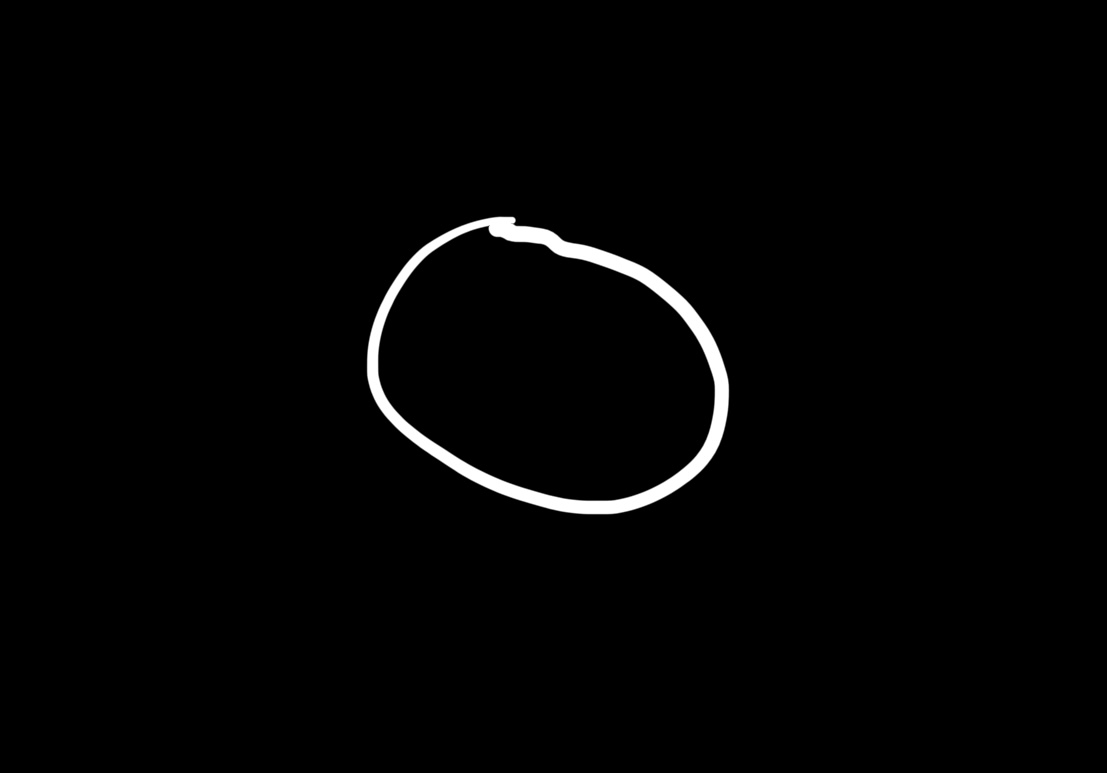
\includegraphics[width=0.4\textwidth]{state-stroke}}
    \subfigure[Rendered state]{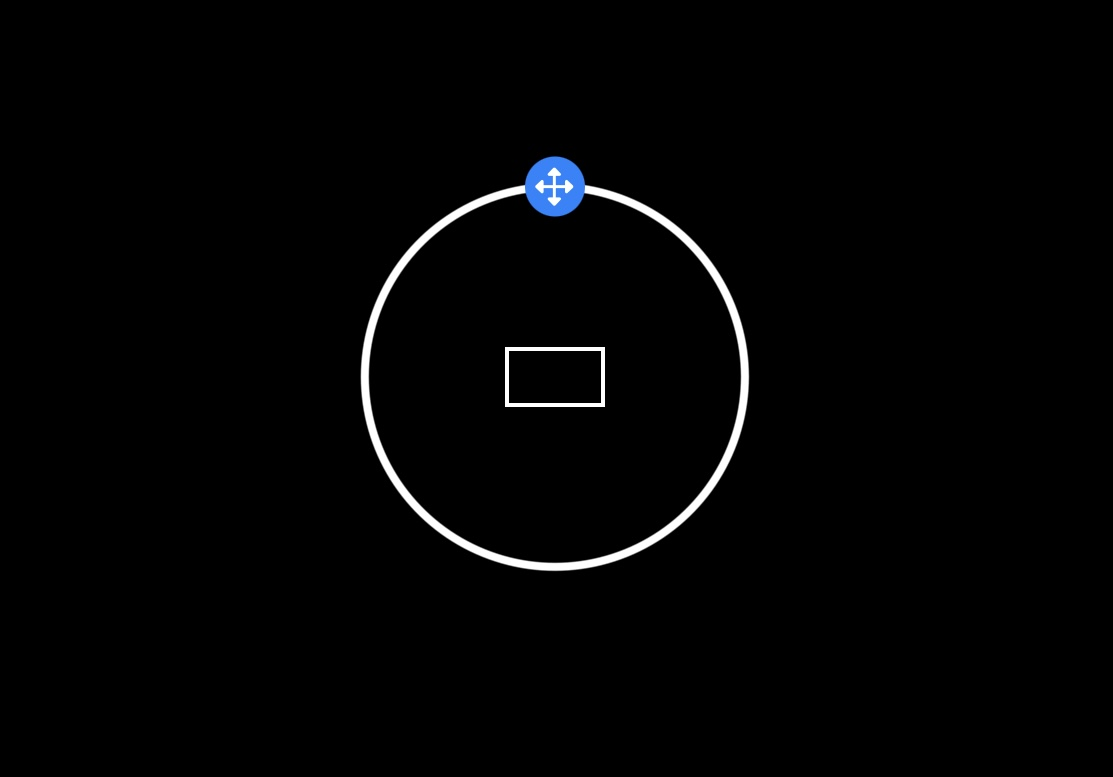
\includegraphics[width=0.4\textwidth]{state}}
    \caption{Example of a state stroke (a) and how it is rendered (b)}\label{state}
\end{figure}

\begin{figure}
    \centering
    \subfigure[]{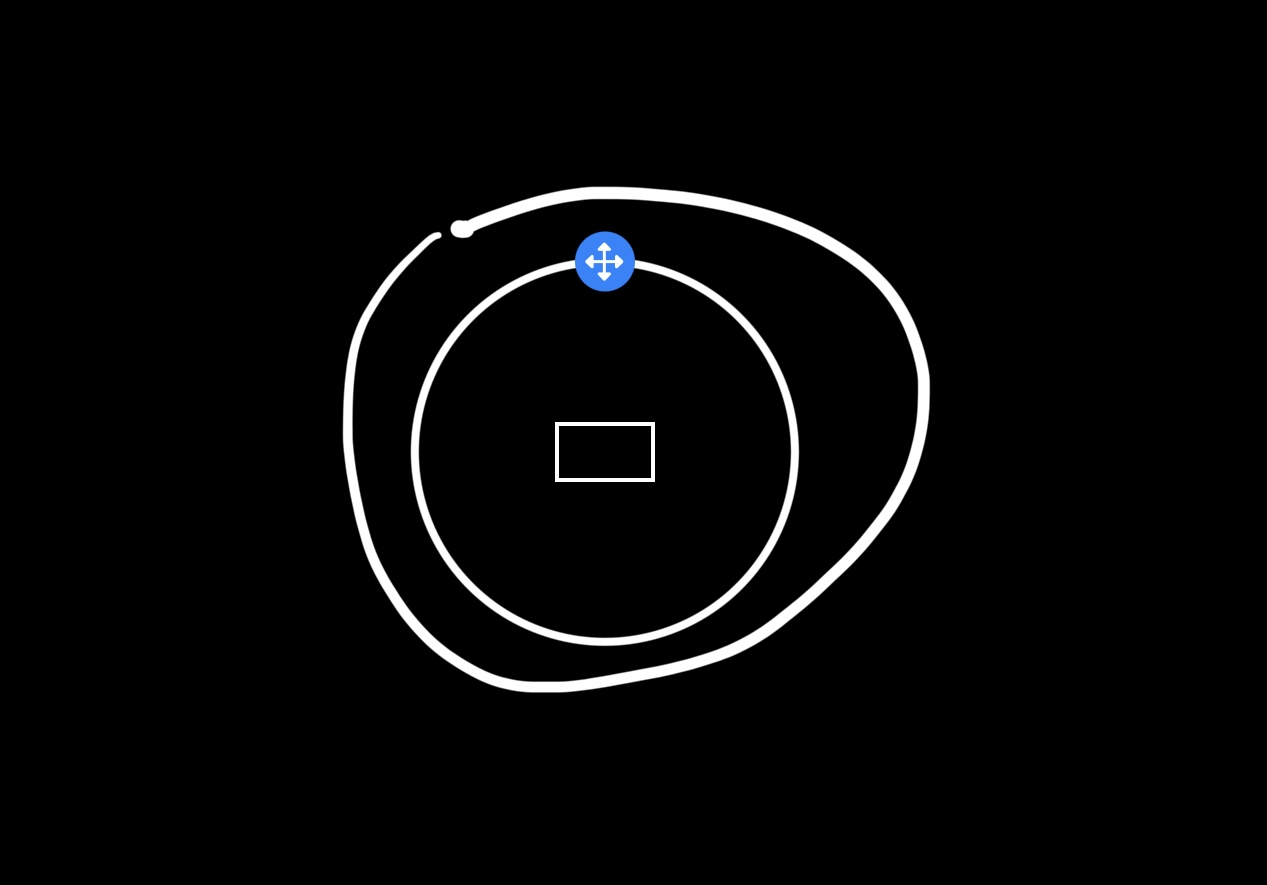
\includegraphics[width=0.4\textwidth]{final-stroke-1}}
    \subfigure[]{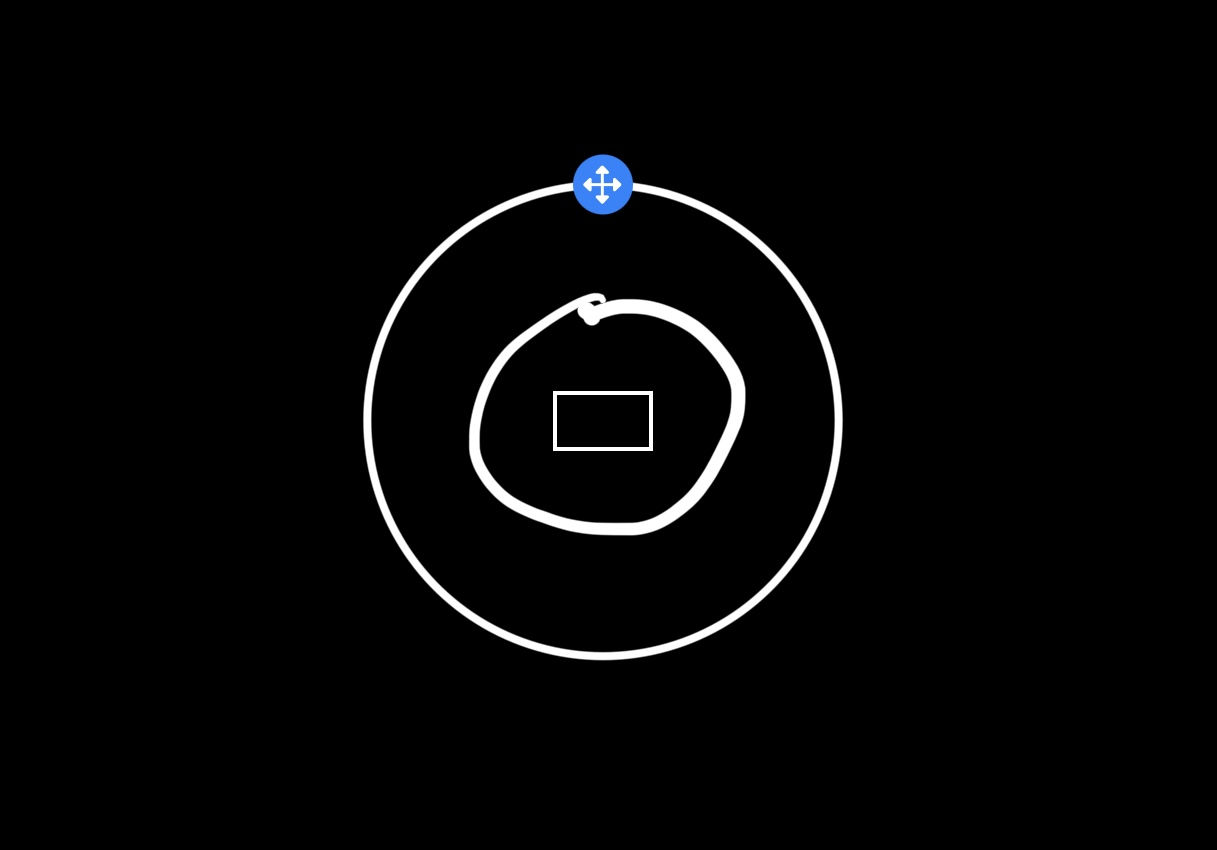
\includegraphics[width=0.4\textwidth]{final-stroke-2}}
    \subfigure[]{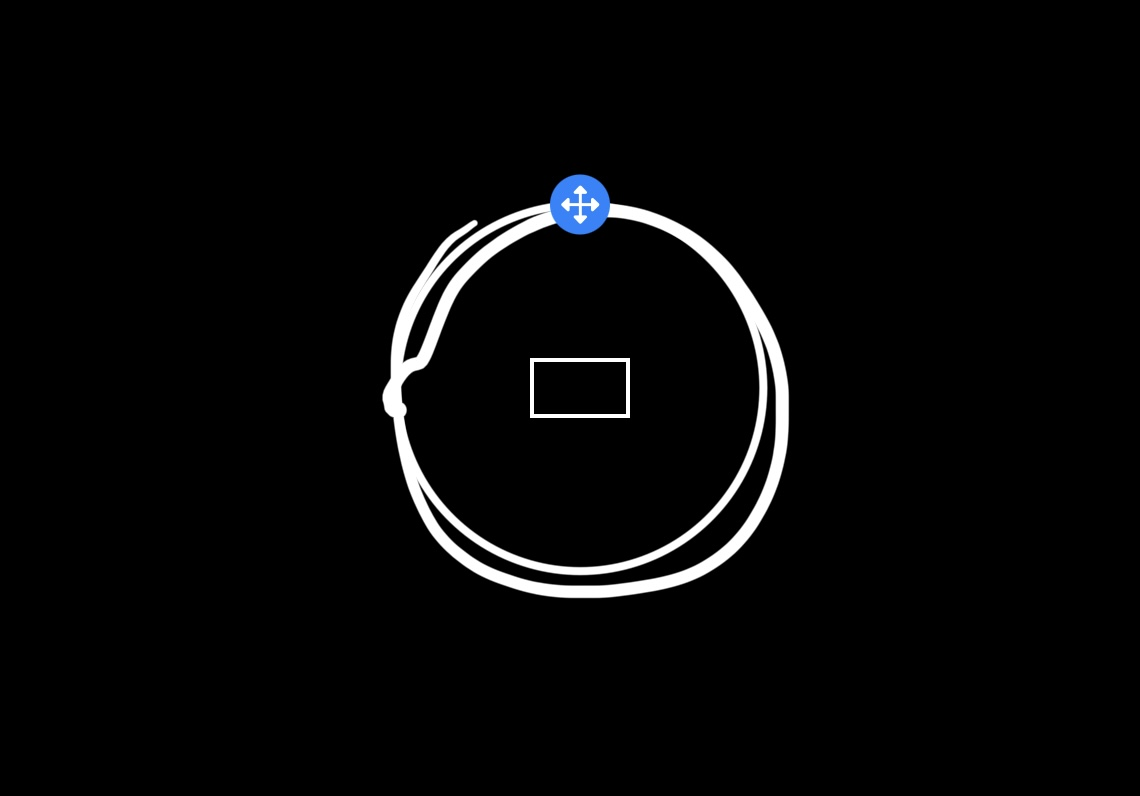
\includegraphics[width=0.4\textwidth]{final-stroke-3}}
    \subfigure[]{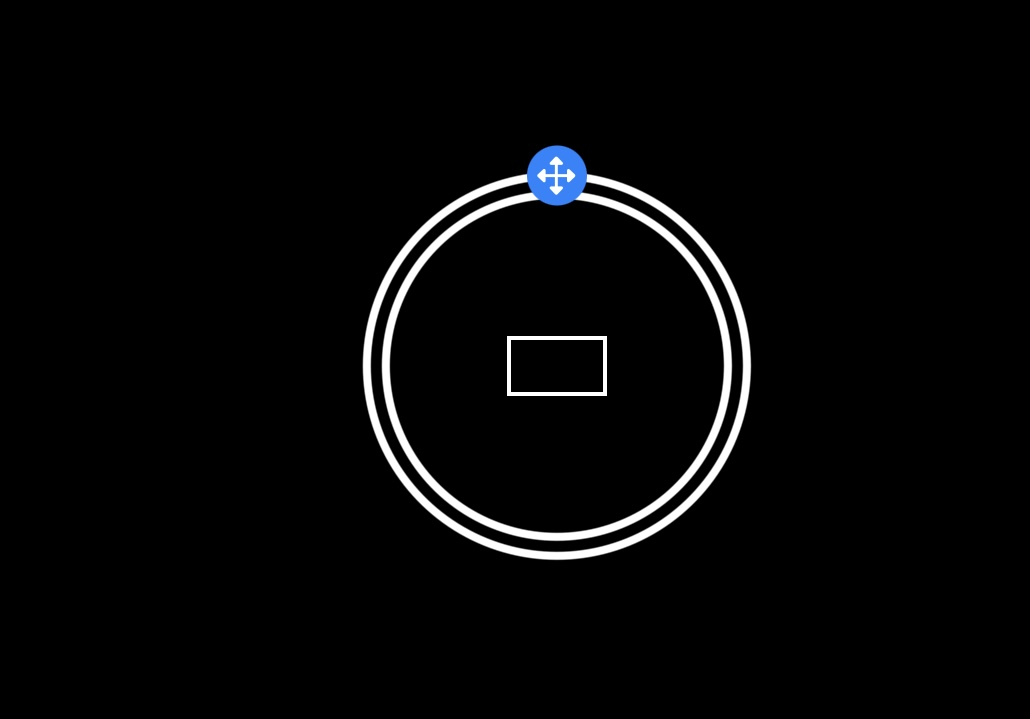
\includegraphics[width=0.4\textwidth]{final-state}}
    \caption{(a), (b), (c) are example strokes that should be rendered as a final state (d)}\label{final-state}
\end{figure}

\subsection{Transition}

A transition is represented as a directed edge between vertices which has a shape of an arrow. The stroke can either be as an arrow or, more conveniently, just a straight line which is faster and easier to draw, especially when the shape must be drawn with a single stroke. Example strokes and a rendered transition are in figure \ref{transition}. Note that the transition can be drawn in no matter which direction. The transition has also a text field positioned above its middle point. Apart from this text field where users can write symbols that the transition should occur on, there is also a button with a plus icon. This button allows users to add multiple symbols to a single transition. Leveraging a delimiter, such as a comma, was also considered but that could inhibit discoverability. Users can easily remove the transition symbols by tapping a cross symbol beside the symbol. To enable drawing a FA with $\epsilon$-transitions there is also a button with $\epsilon$. When it is tapped, $\epsilon$ is added as another symbol for that particular transition. A transition with multiple symbols and with an $\epsilon$-transition are in figure \ref{transition-symbols}. Similar to a state there is a drag button to drag the middle point of a transition. This is especially useful when having multiple states on the same horizontal line with a transition going from the leftmost to the rightmost state.

\begin{figure}
    \centering
    \subfigure[]{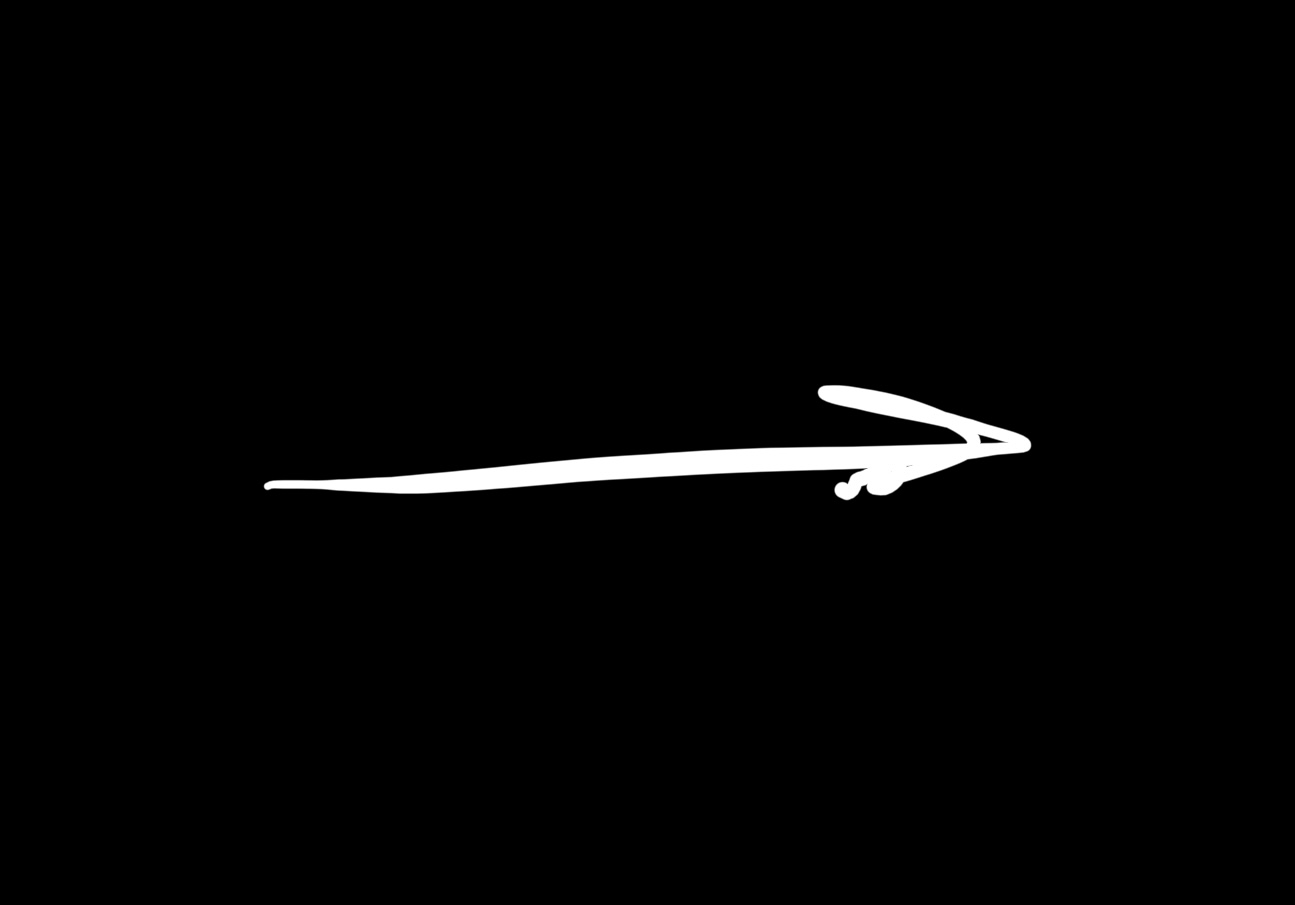
\includegraphics[width=0.4\textwidth]{transition-stroke-1}}
    \subfigure[]{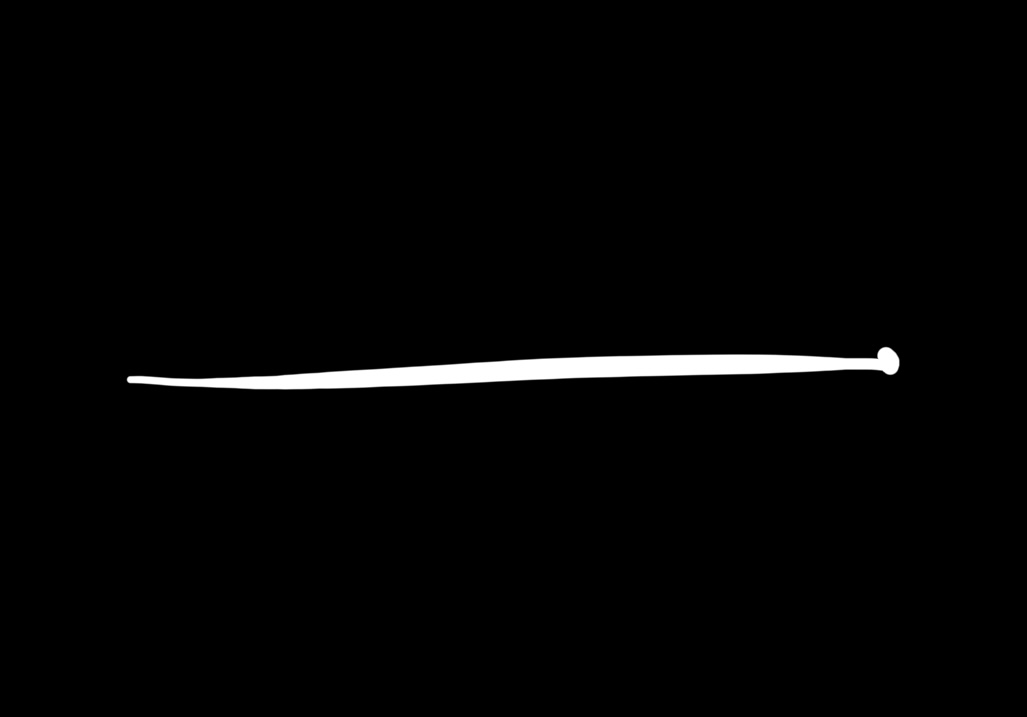
\includegraphics[width=0.4\textwidth]{transition-stroke-2}}
    \subfigure[]{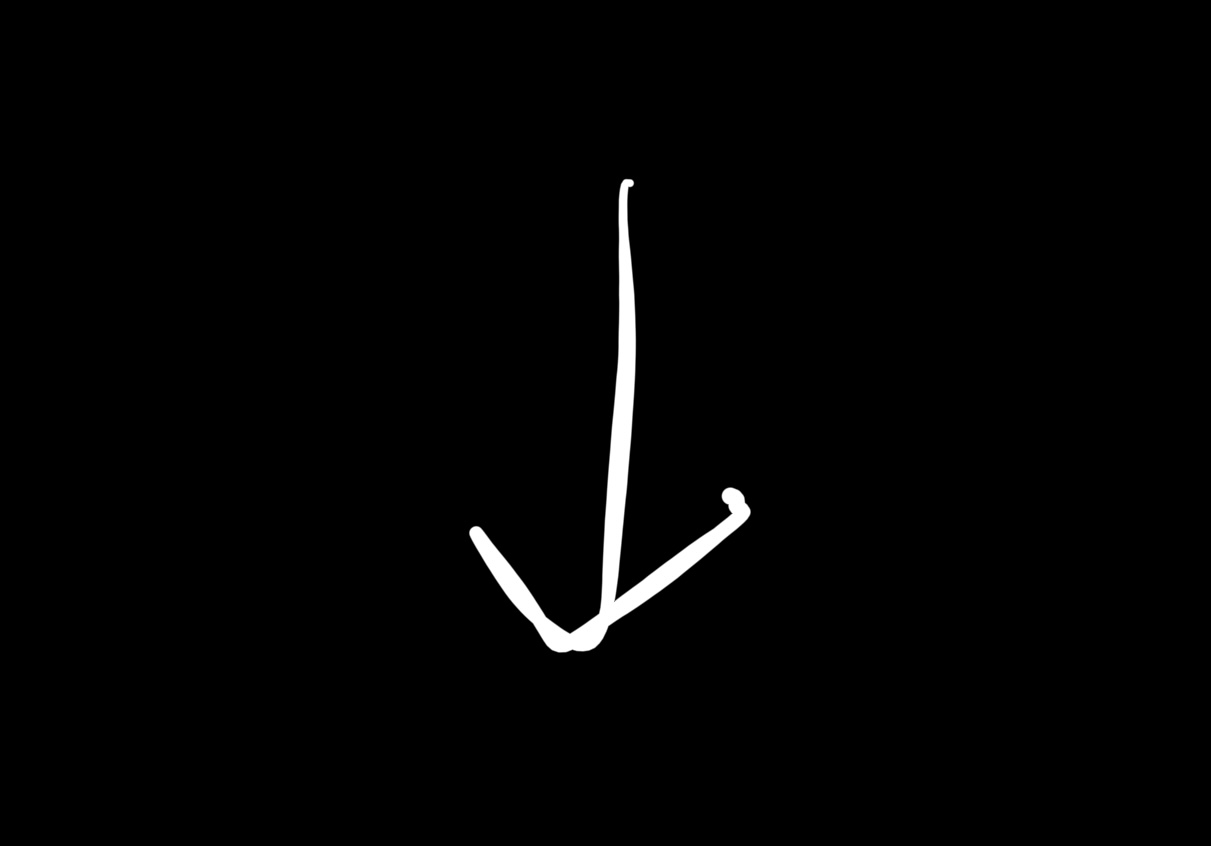
\includegraphics[width=0.4\textwidth]{transition-stroke-3}}
    \subfigure[]{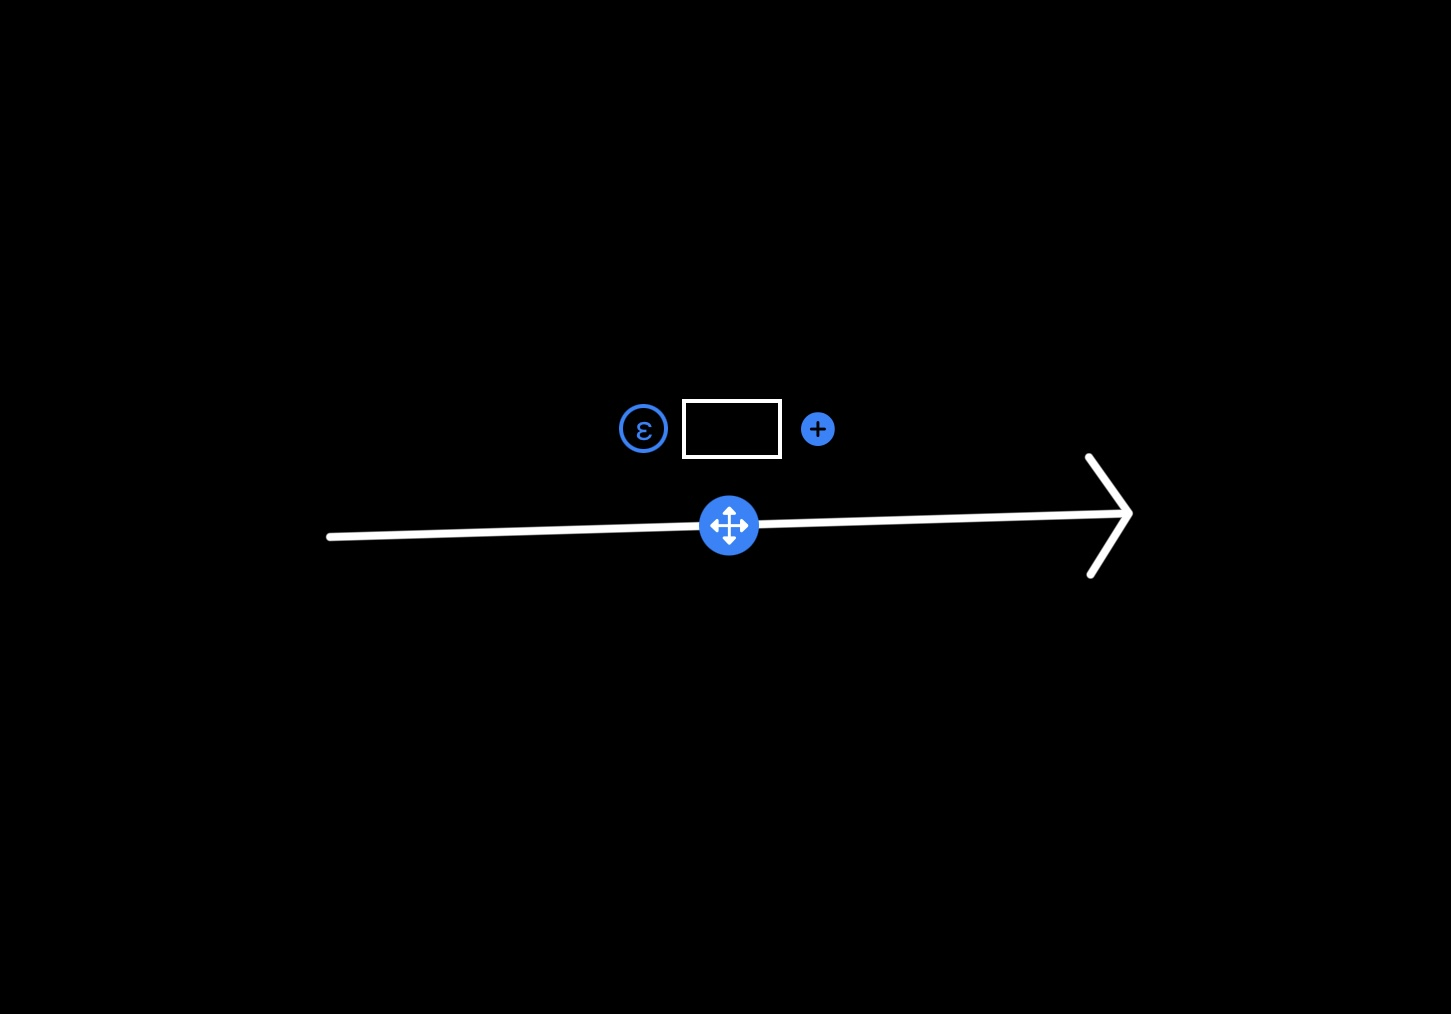
\includegraphics[width=0.4\textwidth]{transition}}
    \caption{(a), (b), (c) are example strokes that should be rendered as a transition (d)}\label{transition}
\end{figure}

\begin{figure}
    \centering
    \subfigure[Transition with multiple symbols]{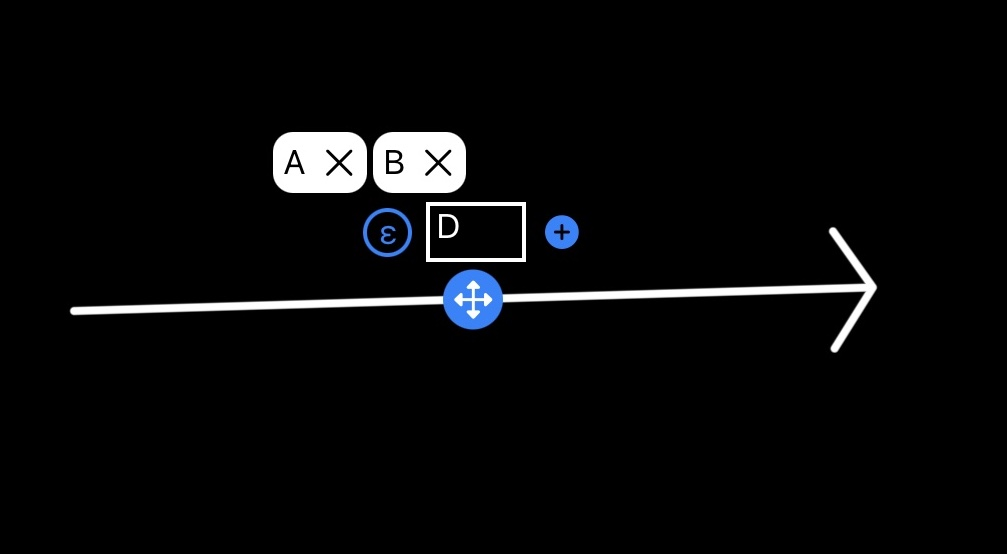
\includegraphics[width=0.4\textwidth]{transition-multiple}}
    \subfigure[$\epsilon$-transition]{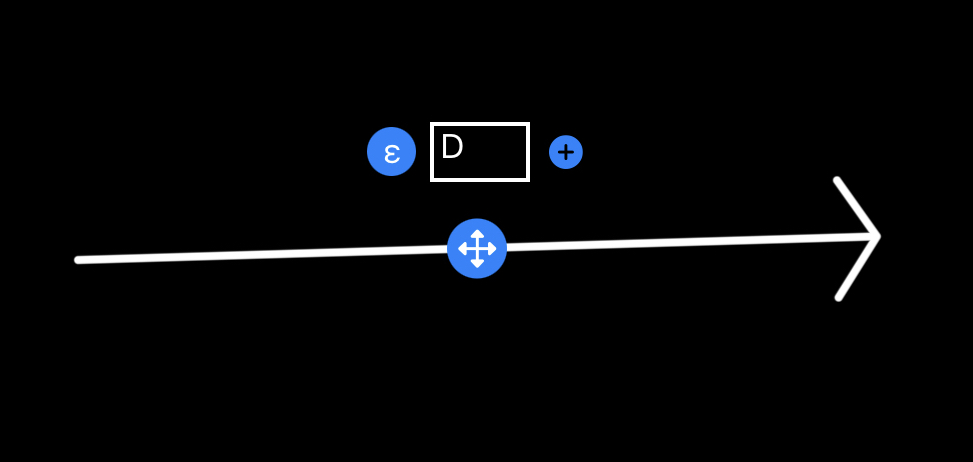
\includegraphics[width=0.4\textwidth]{transition-epsilon}}
    \caption{Transitions with symbols}\label{transition-symbols}
\end{figure}

\subsection{Cycle}

A cycle must be handled differently than a normal transition due to its shape - that means that it must be recognized as a different class in ML model. The business logic tied to a cycle will not be the same, too. Alike a regular transition, it can be drawn in whichever orientation. The ML model should also support multiple variants of a cycle shape to accommodate most of the cycle strokes drawn by users. It should, however, have the same text field, a button for $\epsilon$-transition, as well as multiple transition symbols as a regular transition. The possible strokes and how the cycle should then look like are in figure \ref{cycle}.

\begin{figure}
    \centering
    \subfigure[]{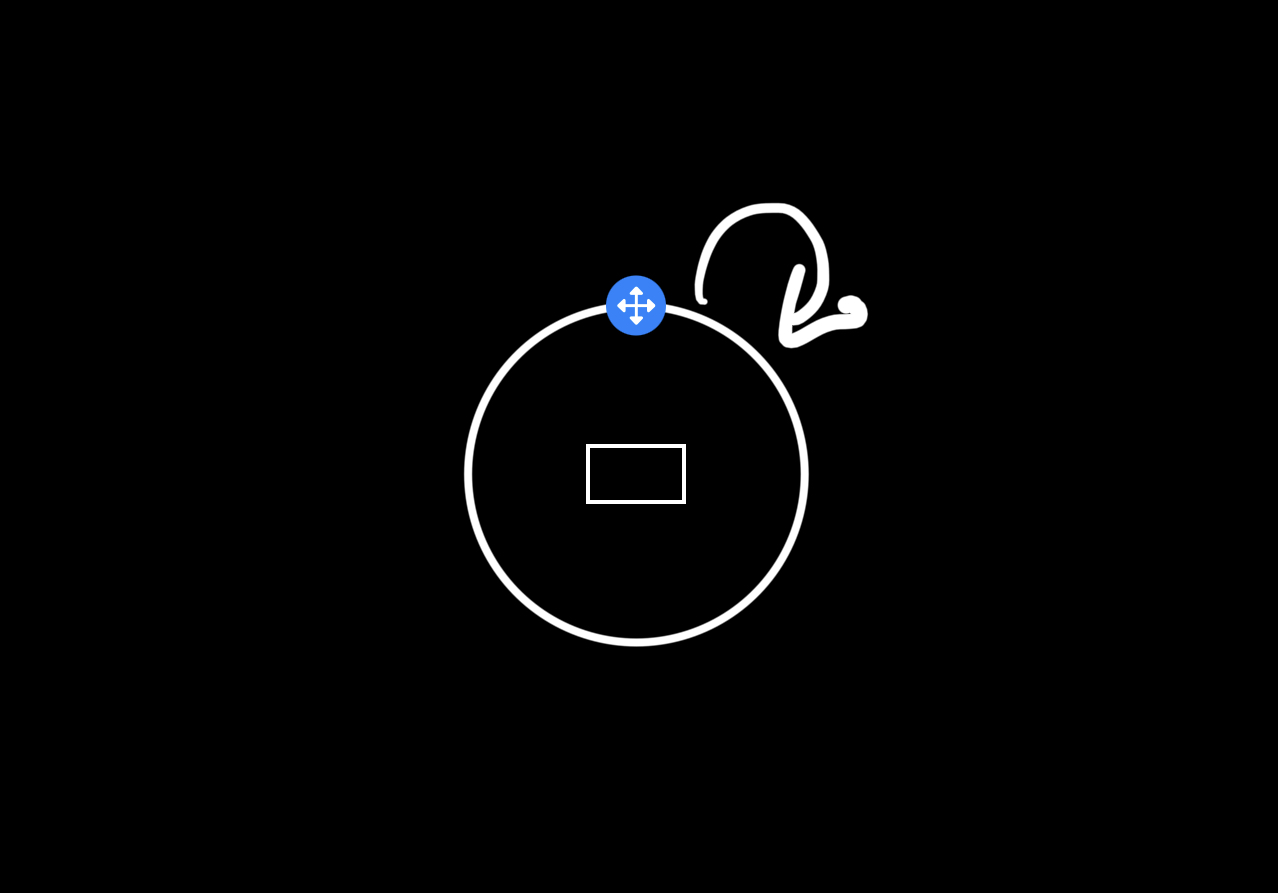
\includegraphics[width=0.4\textwidth]{cycle-stroke-1}}
    \subfigure[]{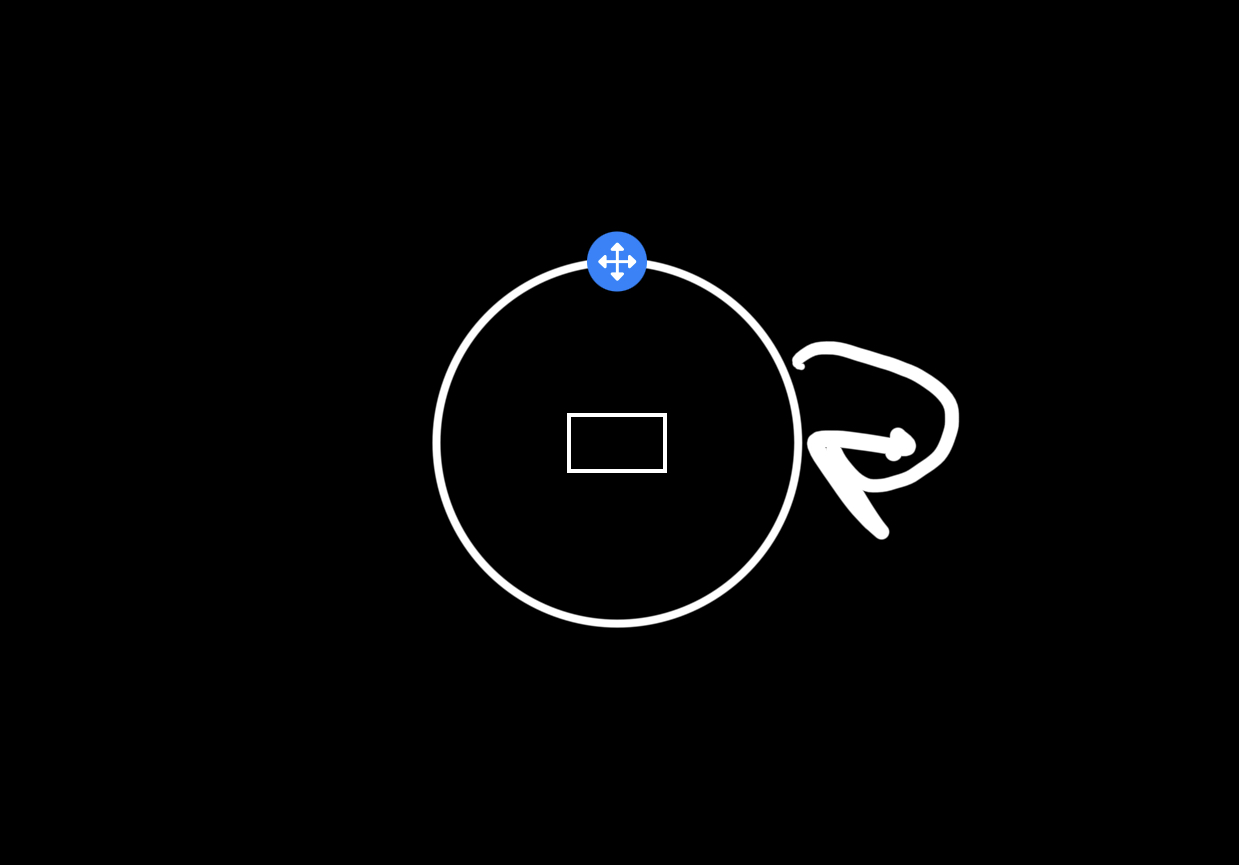
\includegraphics[width=0.4\textwidth]{cycle-stroke-2}}
    \subfigure[]{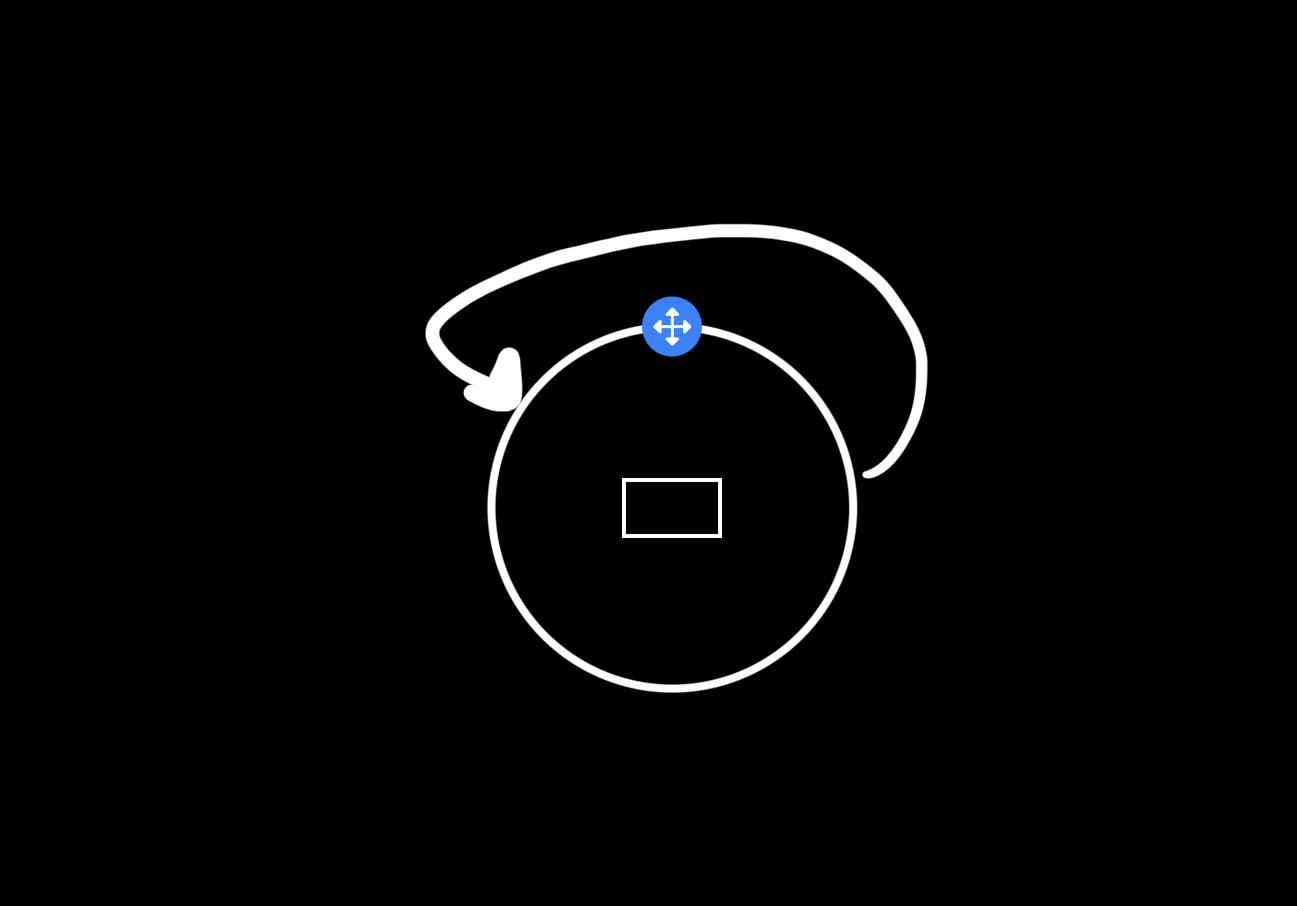
\includegraphics[width=0.4\textwidth]{cycle-stroke-3}}
    \subfigure[]{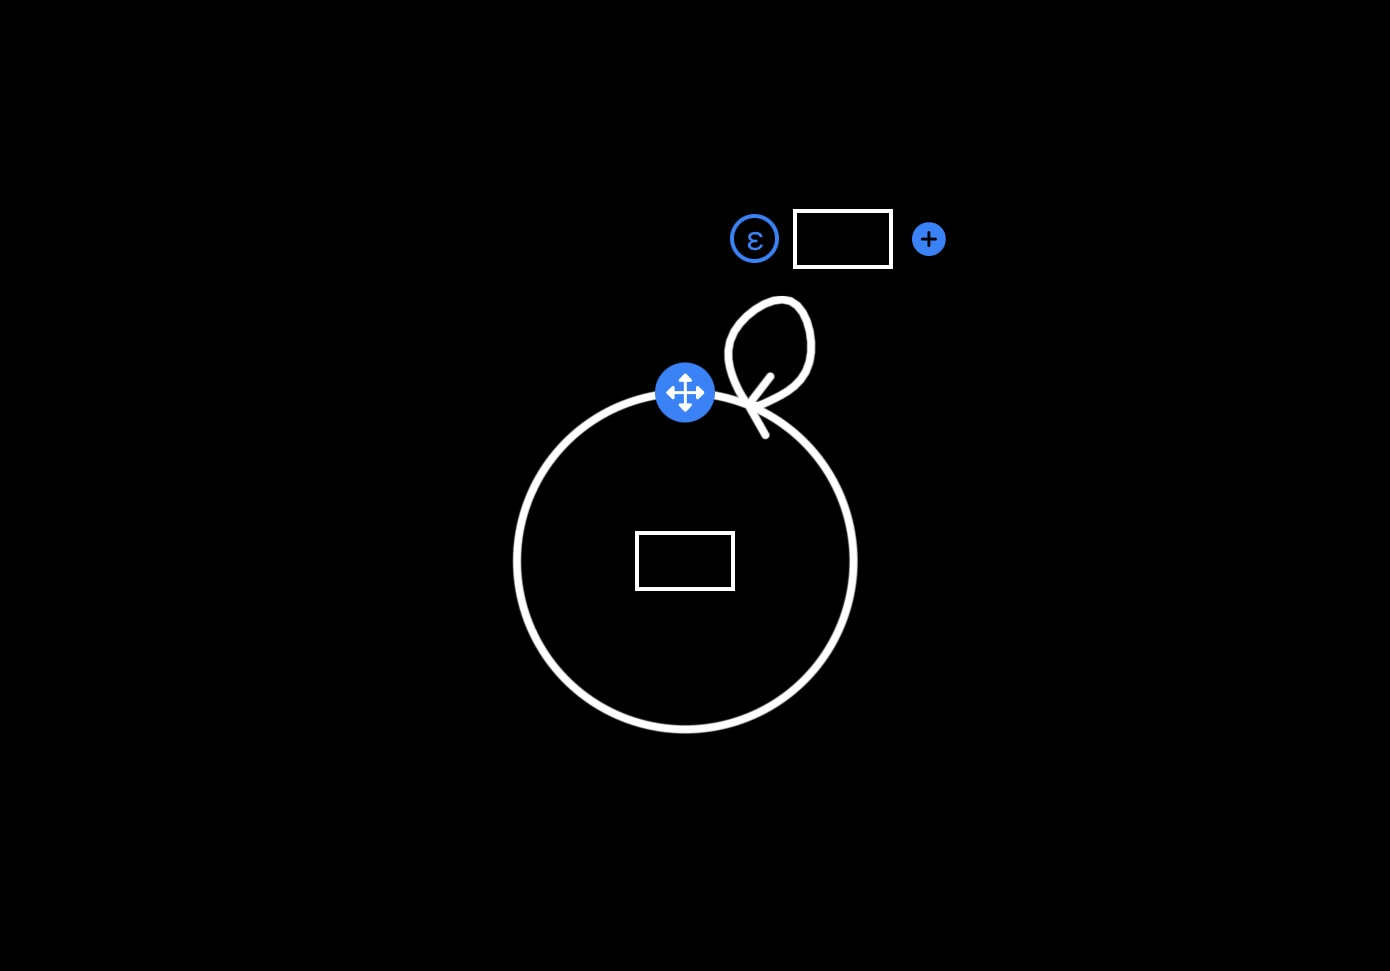
\includegraphics[width=0.4\textwidth]{cycle}}
    \caption{(a), (b), (c) are example strokes that should be rendered as a a cycle (d)}\label{cycle}
\end{figure}

\subsection{Connecting Transitions and States}

So far, I have only described how transitions and states will be recognized in isolation. To create a FA, though, it is necessary to create valid connections between transitions and states. There are multiple cases that the app should support. Similarly to Statemaker \cite{state-maker} it should allow users to create a transition between two existing states. But because the app strives to imitate the experience of using a simple paper, it should be less restrictive and enable creating a transition:
\begin{itemize}
    \item without any state
    \item without a start state
    \item without an end state
    \item with both start and end states
\end{itemize}
For transitions that do not have states on both sides, it must be possible to connect a new state to their end. E.g. if a user draws a state close to a transition's end and it has no state there, it should connect it and make the transition an incoming edge of that state. Note that if the user draws a transition without a start state, it is a valid transition as it will be interpreted as the marking of an initial state.

\subsection{Simulating Input}

The only missing functionality that I have not yet touched upon is simulating input. Considering that a FA is drawn, the user should be able to write their desired input into a text field and see whether the input string has or has not been accepted. That can be done via tapping a button with the title "Simulate". If the FA accepts the input, the output is denoted with the checkmark emoji (\ref{simulate-accept}) and if not, it is denoted with the cross emoji (\ref{simulate-reject}). For convenience, there is a button to erase the last character.

As the currently edited automaton is saved into a custom model specific to the editor app, it is also necessary to convert it to ALT's model and then run the simulation on the ALT model. Before doing so, checks to ensure the automaton is valid are made - such as whether it has an initial state or if all the symbols of the input are in the FA's alphabet. The alphabet itself is constructed by going through the automaton's transitions and adding their symbols. After the conversion is done, the input is simulated on the ALT's FA model and then it is discarded. It is important to note that the ALT model is always recreated when the user simulates a given input.

\begin{figure}
    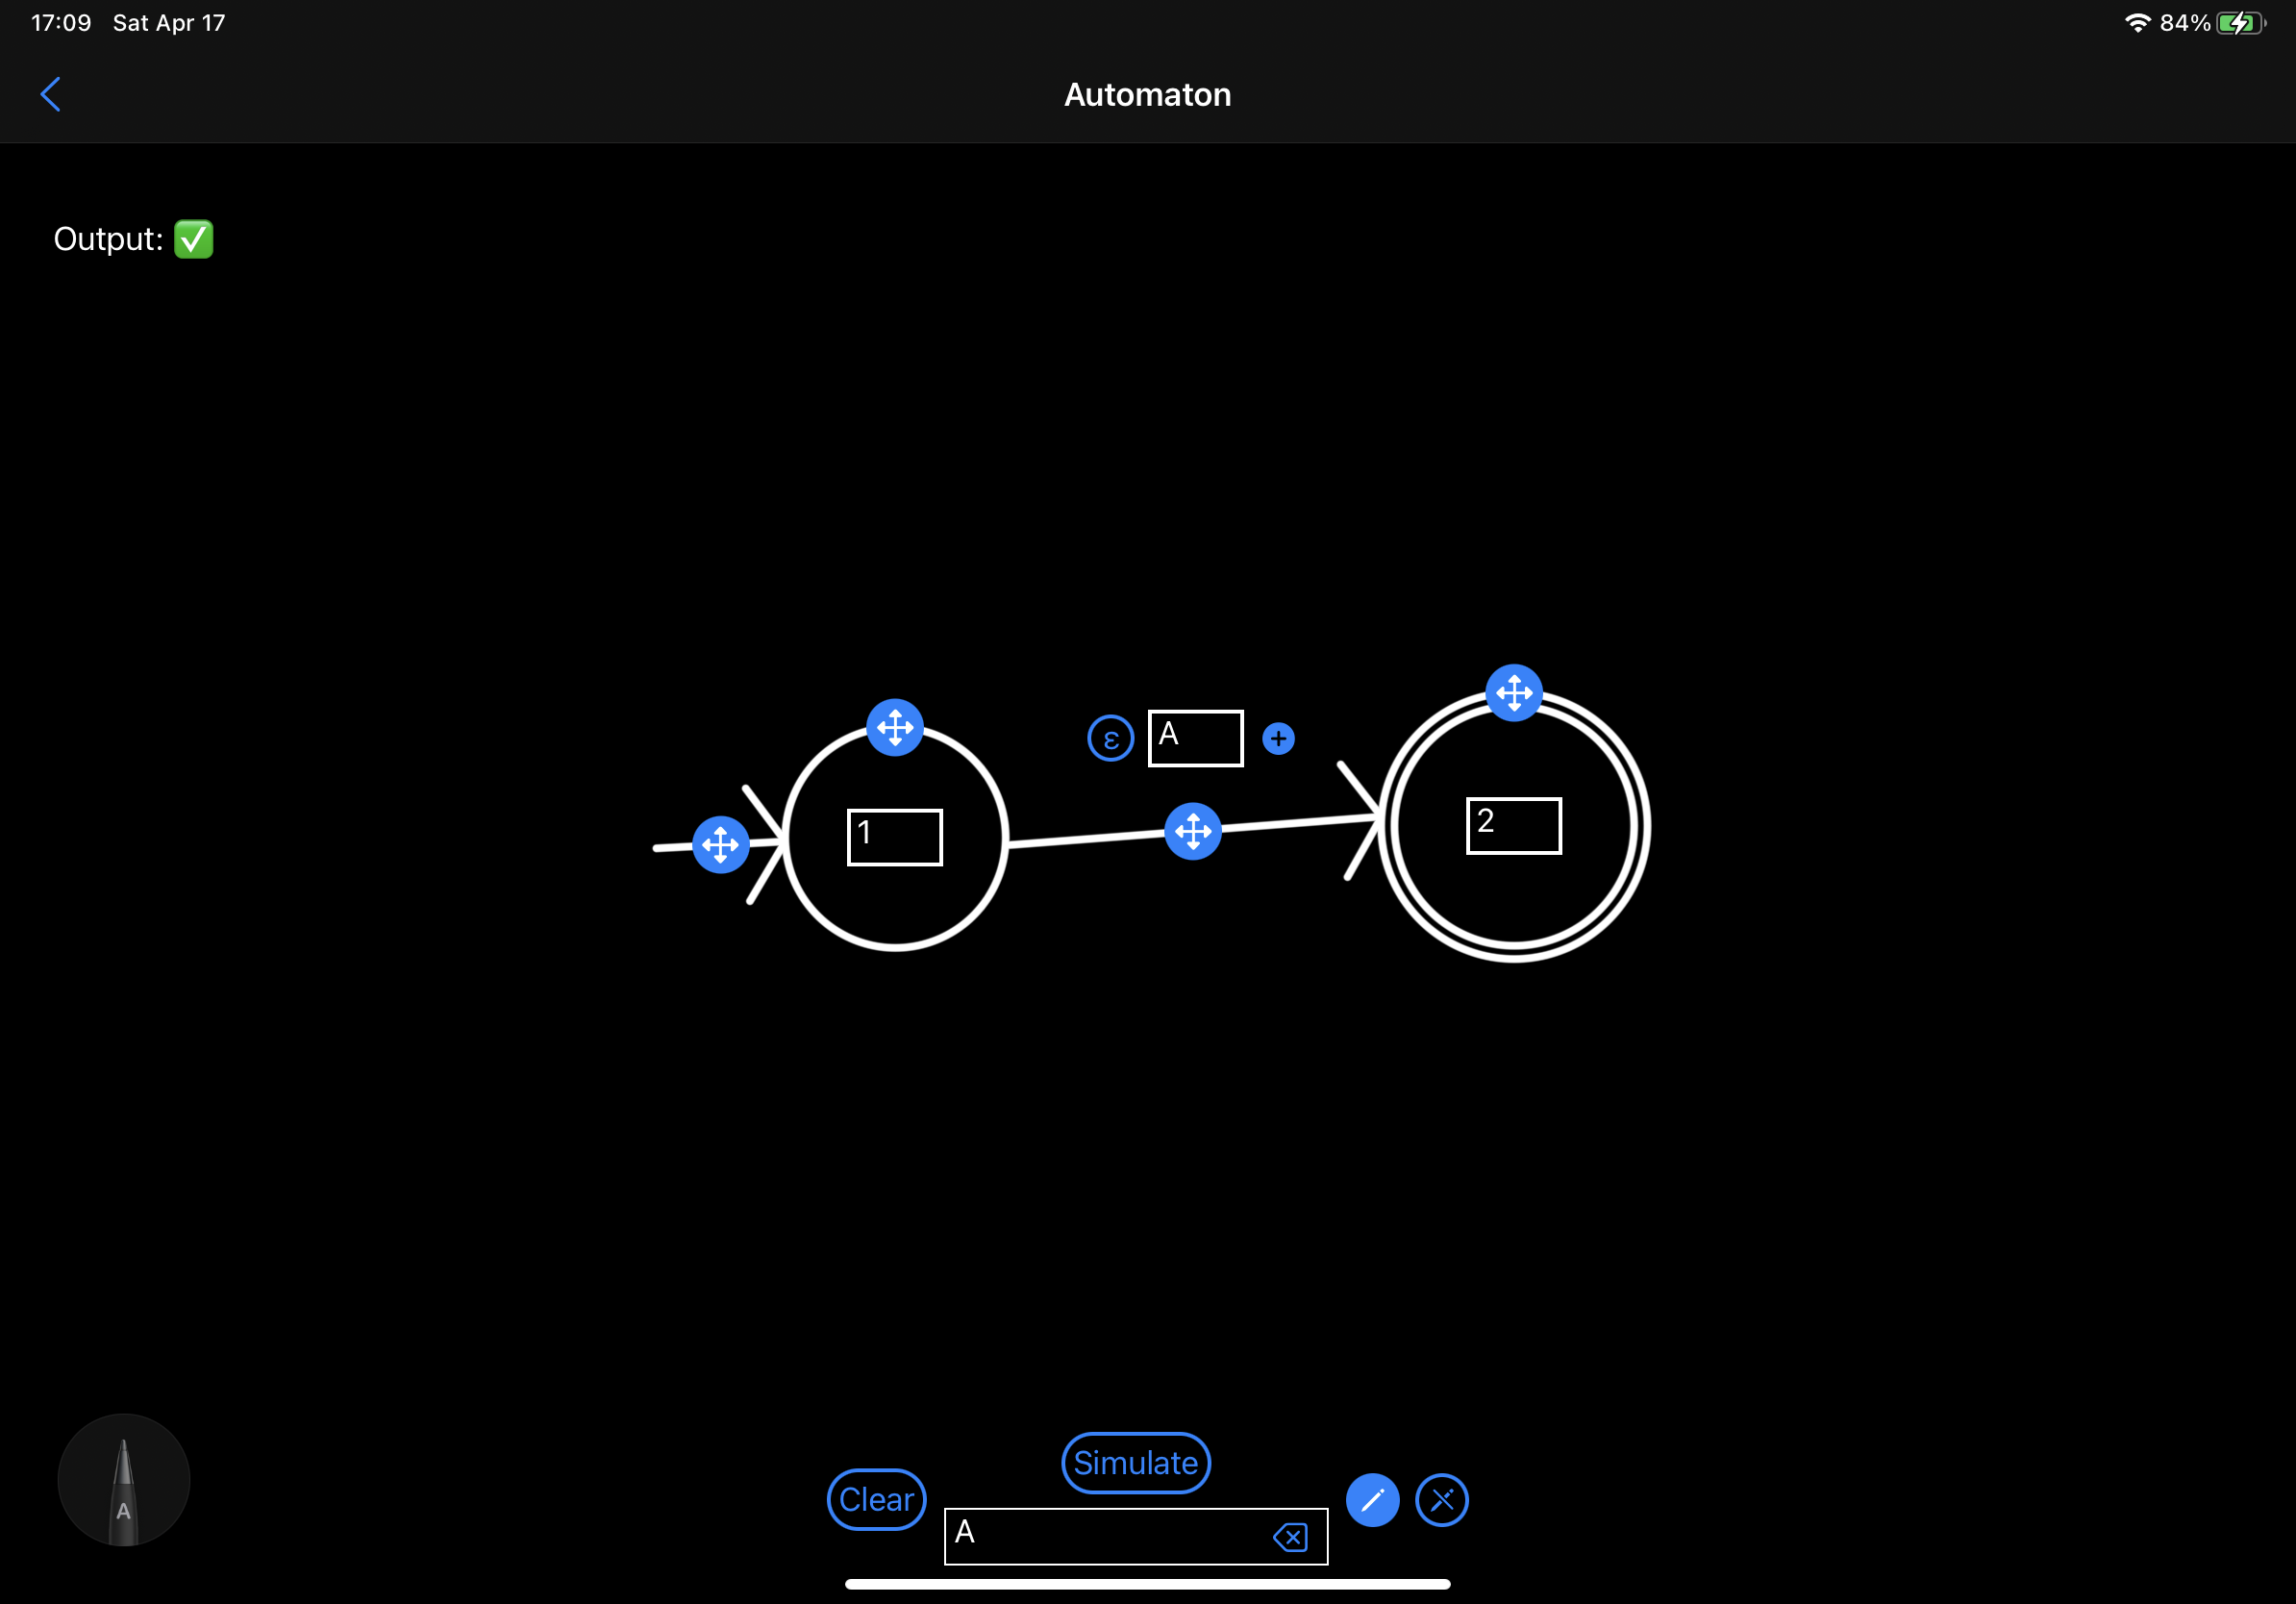
\includegraphics[width=\textwidth]{simulate-accept}
    \caption{Accepted input}\label{simulate-accept}
\end{figure}

\begin{figure}
    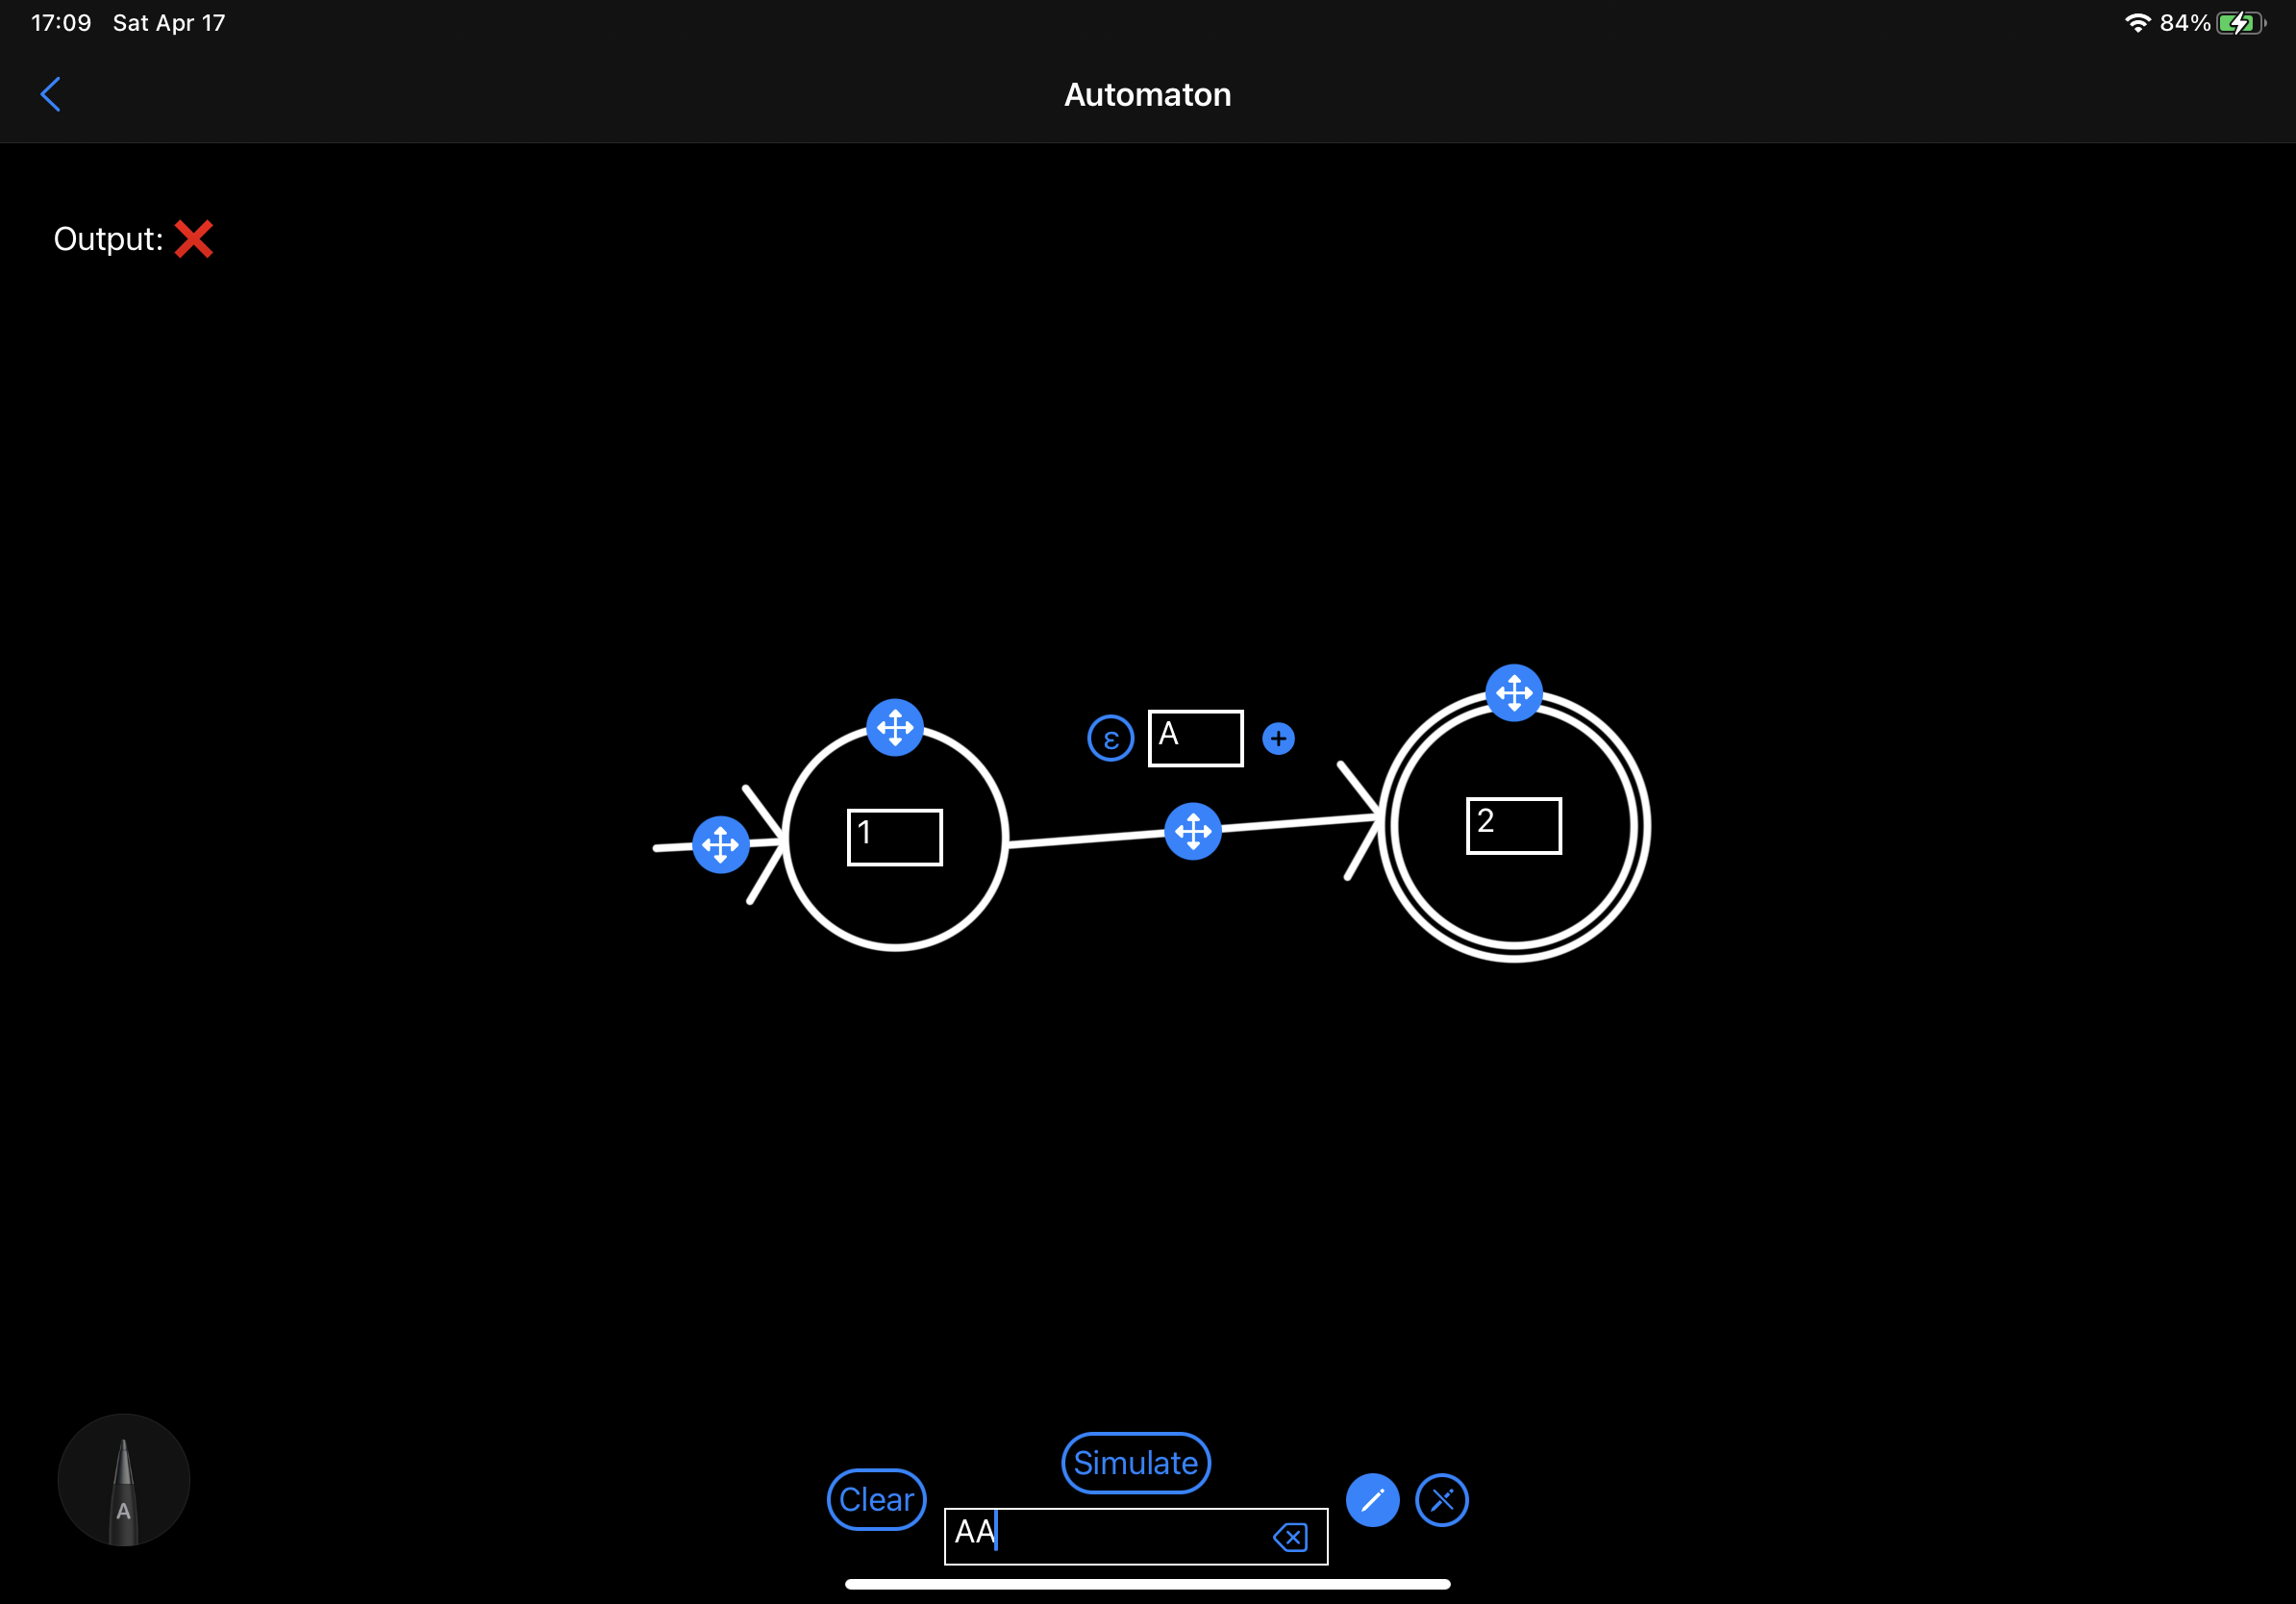
\includegraphics[width=\textwidth]{simulate-reject}
    \caption{Rejected input}\label{simulate-reject}
\end{figure}

\subsection{Erasing}

As you might have noticed in \ref{simulate-accept} and \ref{simulate-reject} there are two buttons right of the input text field. The left is for drawing mode and the right one lets users erase specific elements. If a user made a stroke over an element in the eraser mode, it would be deleted. On the left side there is a "Clear" button that clears the whole canvas whenever it is tapped.

\subsection{Text Fields}

One thing I have purposefully omitted is how the user will interact with the app's text fields. There are two options:
\begin{itemize}
    \item using a keyboard
    \item via Scribble feature
\end{itemize}

Using a keyboard is the standard way of input for text fields. But this breaks the flow of using the Apple Pencil and does not fulfill the goal of imitating real life experience. However, from iOS 14 it is possible to use Apple Pencil for writing in text fields directly \cite{scribble}. This means that it was not necessary to use a custom ML model to achieve the same effect. It does have a drawback and that is the Scribble feature is only available from iOS 14.0 and only if the device's language is in English or Traditional and Simplified Chinese. For other scenarios, users can use a keyboard as a fallback.

\subsection{Document Based Apps}

Users should also be able to save their automata and even share them with other people. The state of the editor should be saved in a document and can be interacted with in what Apple calls document based apps \cite{document-based}. In document based apps it is also possible to save changes done by the user as they happen, ensuring no progress is ever lost.

\chapter{Implementation}
\label{chap:implementation}

I have laid out a basic overview of how the app is designed to look and work. In this chapter I shall go into details of how the most important parts of the app have been implemented. You can also see the source code either in the attached SD card or in the \href{https://github.com/fortmarek/automata-editor}{project's repository}.

\section{ML Model}

A ML model for recognizing FA elements is a core part of the app. I will go over how it has been implemented and integrated.

\subsection{Creating ML Model}

For creating the ML model I have chosen to use turicreate \cite{turicreate} as discussed in chapter \ref{chap:analysis}. The user guide \cite{drawing-classification} describes how to create the ML model for drawing classification using QuickDraw dataset \cite{quickdraw}. This dataset has millions of drawings of various objects, shapes. The shapes do not include, however, arrow and what would resemble a cycle. Therefore, I had to create a custom dataset. To make the ML model as accurate as possible, I have used the same input method for creating the dataset as will be used for drawing the elements in the prototype. For this I have created an MNIST Maker app \cite{mnist-maker}. This app lets you draw shapes with either a finger or Apple Pencil, scales it down to the desired size (I have used 28x28), and converts it to grayscale to make the image as small as possible and it is also what is used when creating the ML Model.

Once I have created a dataset, I could train the ML model. I have used the guide from turicreate and made some modifications like working with grayscale images exclusively (originally, the guide works with RGB images) and specifying which classes to work with. To make iterating on the model easy and quick, I have used a Jupyter notebook \cite{jupyter}. The final Jupyter notebook with the data used is \href{https://github.com/fortmarek/automata-editor-model/}{available on Github}. Once the ML model is trained, one can use turicreate's visualization to see how the ML model worked on the test dataset. In figure \ref{turicreate-visualization} you can see the visualization. From the results it can be seen that the model did not make a mistake in recognizing an arrow but it had mistaken a cycle for a circle and vice versa. This is due to the fact that circles and cycles do have a similar shape.

The final product, once all the commands in the Jupyter notebook are run, is a file \textit{AutomataClassifier.mlmodel}. The extension hints at the fact that it is a ML model that can be used by the CoreML framework.

\subsection{Integration of the ML Model}

To integrate the ML model one has to simply drag and drop the file into Xcode \cite{xcode}, Apple's IDE, to create a reference in the project file. This will automatically bundle the model with the app and synthesize Swift code that can be later leveraged to interact with the model. The code for recognizing a stroke is located in \lstinline{AutomataClassifierService} and the main logic is in a code snippet \ref{automata-classifier}.

\begin{figure}
    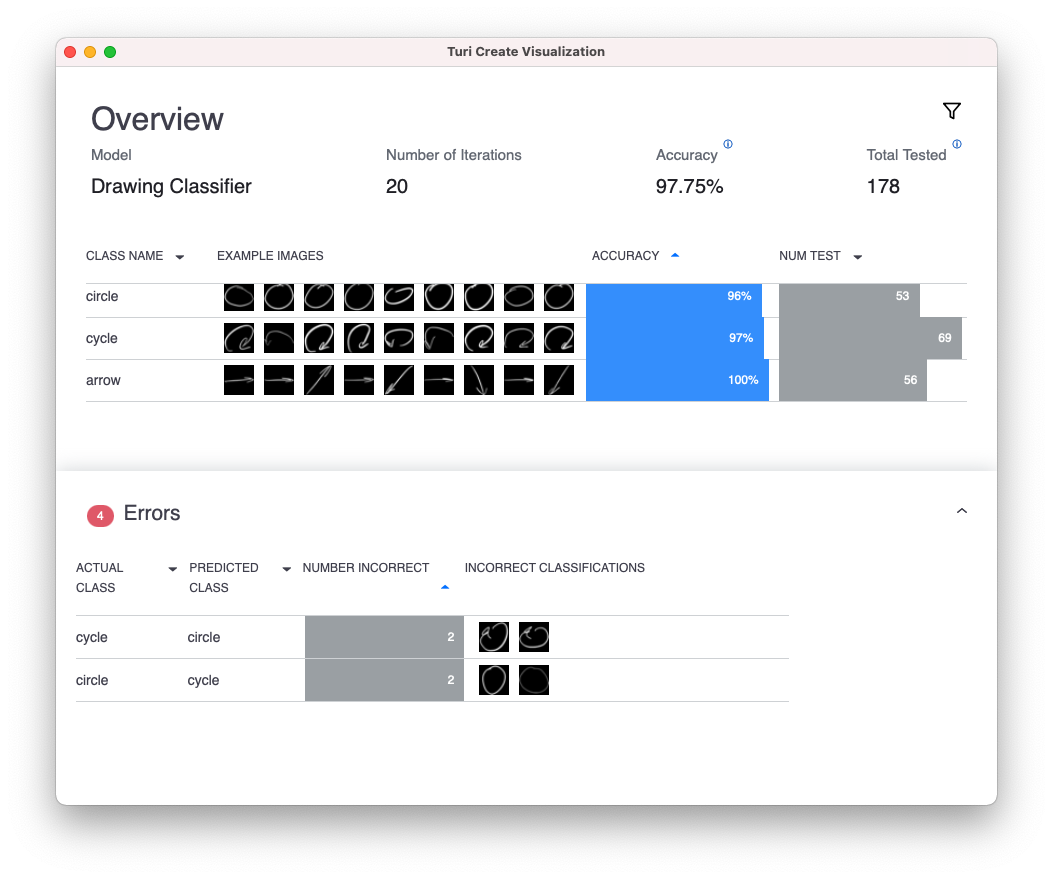
\includegraphics[width=\textwidth]{turicreate-visualization}
    \caption{Test dataset ML model prediction results in turicreate}\label{turicreate-visualization}
\end{figure}

\begin{lstlisting}[caption=Automata classifier, label=automata-classifier]
// Convert stroke to cgImage
// ...
let input = try AutomataClassifierInput(
    drawingWith: cgImage
)
let classifier = try AutomataClassifier(
    configuration: MLModelConfiguration()
)
let prediction = try classifier.prediction(input: input)

guard
    let automataShapeType = AutomatonShapeType(
        rawValue: prediction.label
    )
else { return promise(.failure(.shapeNotRecognized)) }

switch automataShapeType {
case .arrow:
    promise(.success(.transition(stroke)))
case .circle:
    promise(.success(.state(stroke)))
case .cycle:
    promise(.success(.transitionCycle(stroke)))
}
\end{lstlisting}

\section{Drawing FA Elements}

Before FA elements can be recognized, they also must be drawn by the user, converted to a model that can be processed by the \lstinline{AutomataClassifierService} and then re-drawn with a more exact shape once it is known which element the user has made.

\subsection{Canvas}

To enable drawing with the Apple Pencil, Apple offers PencilKit \cite{pencilkit}. One of the components this framework defines is \lstinline{PKCanvasView} - in the documentation described as a "view that captures Apple Pencil input and displays the rendered results in an iOS app" \cite{pkcanvasview}. To use it in SwiftUI, \lstinline{View} I had to wrap it into a view I called \lstinline{CanvasView} conforming to \lstinline{UIViewRepresentable} since \lstinline{PKCanvasView} is only available in UIKit. The instance of \lstinline{CanvasView} was then added to \lstinline{EditorView} which is the main view of the app.

\subsection{Strokes}

When drawing in \lstinline{PKCanvasView} the individual strokes are represented with \lstinline{PKStroke}. It contains all of the available information about the given stroke - such as its bounds, type of ink (\lstinline{PKInt}), and path (\lstinline{PKStrokePath}). In order not to use PencilKit directly and also to make it easier to work with, I wrapped \lstinline{PKStroke} into a custom model \lstinline{Stroke} that contains control points (array of \lstinline{CGPoint}) of \lstinline{PKStroke}. I have not used \lstinline{PKStrokePath} because it contains infinite amount of points. To get only a subset of them one can use a method \lstinline{interpolatedPoints(by: CGFloat)}. The most recent \lstinline{PKStroke} is passed to \lstinline{AutomataClassifierService} and from which an image is created as can be seen in \ref{strokes-conversion} where \lstinline{modelImage()} method simply converts the image from \lstinline{PKDrawing} to grayscale and the desired size.

\begin{lstlisting}[caption=Automata classifier, label=strokes-conversion]
let image = PKDrawing(strokes: [stroke.pkStroke()])
.image(
    from: stroke.pkStroke().renderBounds,
    scale: 1.0
)
.modelImage()
\end{lstlisting}

\subsection{Drawing State}

If the ML classifier predicts that the stroke being analyzed is a state, it is necessary to draw it more precisely than a user. A state is represented as a circle, so to draw it the app needs to know its center and radius. To obtain a center I make an average of all the points available. Once the center is computed, radius is then calculated as an average of distances of all the points from the center. A new stroke can then be created as shown in \ref{circle-init}.

It is also necessary to connect a state to an existing transition. There is a method for this called \lstinline{closestTransitionWithoutEndState} that, as the name suggests, finds the closest transition that does not have an end state. If such a transition exists, a center is moved in the direction of the tip of the transition, so they have a single intersection point.

A final state is marked with a double circle. Therefore, if a stroke is a state, before making a new one I check whether a center of a different state is contained in a frame of the new state. If it is so, then the state is marked as final and a new circle around the previous one is made and the state is denoted in the internal state as a final one.

\begin{lstlisting}[caption=Circle stroke, label=circle-init]
extension Array where Element == CGPoint {
    static func circle(
        center: CGPoint,
        radius: CGFloat
    ) -> Self {
        stride(from: CGFloat(0), to: 362, by: 2).map { index in
            let radians = index * CGFloat.pi / 180
            
            return CGPoint(
                x: CGFloat(center.x + radius * cos(radians)),
                y: CGFloat(center.y + radius * sin(radians))
            )
        }
    }
}
\end{lstlisting}

\subsection{Transition}

To draw a transition I take its first and last point (tip point). At the tip point two additional lines must be made, so the final shape looks like an arrow. For this I needed vectors, so it works for whichever orientation. Vectors are not offered by any of the bundled frameworks, so I have heavily inspired my implementation from a repository called VectorMath \cite{vectormath}. Once vectors were available, I was able to compute a perpendicular vector to the line from the start point to the tip point that has one common point with that line and that is a point on the transition's line in a pre-defined distance from the tip point. The bottom and top points are then on that vector with a pre-defined distance from the line as well. To add additional points, top and bottom vectors are created by connecting top and bottom points with the tip point as in \ref{transition-points}.

Similarly to states, it is necessary to handle the case when a new transition should be connected to an existing state. Firstly, the closest states to the start point and the tip point are computed. Then the closer one is chosen as a start state or end state, respectively - if the distance is smaller than a given threshold.

\begin{lstlisting}[caption={Computation of top and bottom points, vectors}, label=transition-points]
let vector = Vector(flexPoint ?? startPoint, tipPoint)
let anchorPoint = vector.point(
    distance: -arrowSpan / 3, 
    other: tipPoint
)
let perpendicularVector = vector.rotated(by: .pi / 2)
let topPoint = perpendicularVector.point(
    distance: -arrowSpan / 2,
    other: anchorPoint
)
let bottomPoint = perpendicularVector.point(
    distance: arrowSpan / 2,
    other: anchorPoint
)
let topVector = Vector(tipPoint, topPoint)
let bottomVector = Vector(tipPoint, bottomPoint)
\end{lstlisting}

\subsection{Cycle}

The last class that the ML model classifies and that has not been discussed how to draw is a cycle. A cycle is different from a state and a transition since it can not exist without being connected to a state. If there is no state to connect it to, the stroke is just erased. Otherwise, once the closest state is found the cycle's shape can be created. Its shape is more complicated than the previous - but it is possible to use PencilKit's behavior that smoothes out a curve based on the points given. Thus, to recreate it I used the point at the intersection with the state and the state's center in \ref{cycle-init}.

\begin{lstlisting}[caption=Cycle stroke, label=cycle-init]
extension Array where Element == CGPoint {
    static func cycle(
        _ point: CGPoint,
        center: CGPoint
    ) -> Self {
        let vector = Vector(point, center)
        let topPoint = vector.point(distance: -70, other: point)
        let startToTopVector = Vector(point, topPoint)
        let finalPoint = startToTopVector
            .rotated(by: .pi * 0.4)
            .point(distance: 5, other: point)
        return [
            point,
            startToTopVector
                .rotated(by: -.pi / 3)
                .point(distance: 10, other: point),
            startToTopVector
                .rotated(by: -.pi / 4)
                .point(distance: 40, other: point),
            topPoint,
            startToTopVector
                .rotated(by: .pi / 4)
                .point(distance: 40, other: point),
            startToTopVector
                .rotated(by: .pi / 3)
                .point(distance: 10, other: point),
        ] + .arrow(
            startPoint: finalPoint,
            tipPoint: point,
            arrowSpan: 30
        )
    }
}
\end{lstlisting}

\section{ALT Integration}

ALT integration has been discussed both in chapter \ref{chap:analysis} and chapter \ref{chap:design}. 

\subsection{Source Code}
In chapter \ref{chap:design} I have already hinted that I had first attempted to integrate the source code directly. Swift Package Manager is a package manager by Apple that is integrated right in Xcode \cite{spm}. Therefore, if I was able to use that for building ALT, others could benefit from this and it would make the integration seamless. To create a package via Swift Package Manager one must create \lstinline{Package.swift} manifest where the products and other targets are defined. It is also possible to define C++ headers and flags. But the headers in the ALT source code point to already built modules by CMake. This means that when I tried to build the code, I got compiler errors about \lstinline{#include} directive pointing to non-existent headers. This was possible to circumvent by modifying \lstinline{#include} directives to point to existing locations, instead of pointing to the built modules. But doing so would be a maintenance burden. Thus, I have decided not to integrate the source code directly but rather only frameworks built with CMake.

\subsection{Headers}
ALT's current version only supports \lstinline{gcc} compiler. But to build frameworks for iOS it is necessary to use clang \cite{clang}. At the time of writing ALT is not compilable with the standard library in clang since ALT uses some C++20 features that are only implemented in gcc - for example \lstinline{lexicographical_compare_three_way}, among others. It is possible to point clang to headers from gcc via \lstinline{-cxx-isystem} flag and \lstinline{-stdlib=libstdc++} that tells clang to parse the headers as \lstinline{libstdc++} instead of \lstinline{libc++}. But this is not possible to do since Xcode 10 has dropped support for \lstinline{libstdc++} and all C++ projects must use \lstinline{libc++} standard library. In the future, it should be feasible to use the current version of ALT with some newer version of clang as they add support for C++20 features. ALT has only recently started using C++20 features, so to fix this issue, a new branch \lstinline{libc++-17} was created by Jan Trávníček from a commit from before C++20 features have been introduced to the codebase.

\subsection{CMake}

There is support for building for iOS platform in CMake directly. To save some upfront work I have used ios-cmake toolchain file that builds on top of CMake and makes the setup easier \cite{ios-cmake}. An example of how to build a framework for \lstinline{OS64} (iOS) is in \ref{cmake-build}. The same could then be done for a simulator by specifying \lstinline{SIMULATOR64}. This way two different frameworks are built. For combining multiple frameworks with different architectures there is XCFramework \cite{xcframework}. I have created a small shell script in \ref{xcframework-bundle} that creates a new XCFramework from frameworks necessary for the editor app. The built XCFrameworks could then be moved to Xcode.

\begin{lstlisting}[caption=CMake build instructions, label=cmake-build]
mkdir build
cd build
cmake .. -G Xcode \
-DCMAKE_TOOLCHAIN_FILE=../../ios.toolchain.cmake -DPLATFORM=OS64
cmake --build . --config Debug
\end{lstlisting}

\begin{lstlisting}[caption=XCFramework shell script, label=xcframework-bundle]
#!/bin/sh
modules=(
    "alib2std" \
    "alib2measure" \
    "alib2abstraction" \
    "alib2common" \
    "alib2xml" \
    "alib2str" \
    "alib2data" \
    "alib2algo" \
)
for module in "${modules[@]}"
do
    xcodebuild -create-xcframework \
    -framework ../build/$module/Debug-iphoneos/$module.framework \
    -framework \
    ../simulator/$module/Debug-iphonesimulator/$module.framework \
    -framework \
    ../arm64/$module/Debug-iphonesimulator/$module.framework \
    -output $module.xcframework
done
\end{lstlisting}

\subsection{Objective-C and Swift Wrappers}

With XCFrameworks in Xcode, the next step was to write wrappers, so the C++ frameworks could be used in Swift code. As mentioned in chapter \ref{chap:design} it is not possible to interact with C++ code from Swift directly - for this Objective-C++ wrappers had to be written, exposing only Objective-C in its interface. To better encapsulate the wrappers I have also created a separate module \lstinline{SwiftAutomataLibrary}. The most important part in Objective-C is present in \lstinline{NFA_objc} that interacts with ALT's \lstinline{EpsilonNFA} class. Its interface is in \ref{nfa-objc-interface}. It is initialized with all necessary data to create the underlying automaton and has one method that takes a list of symbols for input and returns \lstinline{bool} based on whether the input was accepted or rejected. All necessary conversions are done in the implementation file. E.g. states are passed to \lstinline{NFA_objc} as \lstinline{NSArray *} where the individual elements are \lstinline{NSString *}. This had to be converted to \lstinline{ext::set<std::string>}.

\begin{lstlisting}[caption={NFA\_objc interface}, label=nfa-objc-interface]
- (instancetype)init: (NSArray *) states
    inputAlphabet:(NSArray *) inputAlphabet
     initialState:(NSString *) initialState
      finalStates:(NSArray *) finalStates
      transitions: (NSArray *) transitions;
- (bool)simulate: (NSArray *) input;
\end{lstlisting}

The wrapper between Swift and Objective-C was then more straightforward as conversions between a lot of types - such as \lstinline{NSArray *} and \lstinline{Array} - are done automatically. It also would be possible to use \lstinline{NFA_objc} directly but to have better control I have created \lstinline{NFA} as a simple Swift struct. This is the only part that was made public in the SwiftAutomataLibrary module.

\section{App State}

I have already explained how the FA elements are recognized, rendered and how the ALT C++ code is bridged to Swift. Now I would like to explain a little bit more the internal state of the app - of which the most substantial part is located in \lstinline{EditorStore.swift}.

\subsection{FA Models}

There are two FA models - \lstinline{AutomatonTransition} and \lstinline{AutomatonState}. Notably, a cycle does not have its separate model but is rather an \lstinline{AutomatonTransition}. But since it is rendered differently, it must be recognizable from a normal transition - for this there is \lstinline{enum TransitionType} that has two types - \lstinline{regular} and \lstinline{cycle}. \lstinline{AutomatonTransition} can be seen in \ref{transition-model}. The \lstinline{id} property is generated for each element at the moment when it is created, so it is easily distinguishable. The same is done for \lstinline{AutomatonState}.  Apart from what you see in the code snippet \lstinline{AuomatonTransition} has a set of computed properties like \lstinline{stroke}. Computed properties are great for keeping the state of the model consistent and should be used whenever a property's value can be safely and in a performant way derived from other properties of that model. \lstinline{AutomatonState} is similar to the transition with some specific properties like \lstinline{isFinalState} denoting whether a state is final or \lstinline{center} used to determine a state's center.

\begin{lstlisting}[caption={Transition model}, label=transition-model]
struct AutomatonTransition: Equatable, Identifiable, Codable {
    enum TransitionType: Equatable, Hashable, Codable {
        case cycle(
            CGPoint, 
            center: CGPoint, 
            radians: CGFloat
        )
        case regular(
            startPoint: CGPoint, 
            tipPoint: CGPoint, 
            flexPoint: CGPoint
        )
    }
    let id: String
    var startState: AutomatonState.ID?
    var endState: AutomatonState.ID?
    var currentSymbol: String = ""
    var symbols: [String] = []
    var includesEpsilon: Bool = false
    var type: TransitionType
    var currentFlexPoint: CGPoint? = nil
}
\end{lstlisting}

\begin{lstlisting}[caption={State model}, label=state-model]
struct AutomatonState: Equatable, Identifiable, Codable {
    let id: String
    var name: String = ""
    var isFinalState: Bool = false
    var center: CGPoint
    let radius: CGFloat
    var currentDragPoint: CGPoint
}
\end{lstlisting}

\subsection{Simulating Input}

Simulating the automaton's input is the main feature of the prototype. Once a user taps on "Simulate" button, \lstinline{simulateInput} action is triggered. There some preliminary checks are made - such as whether the FA has an initial state (\ref{initial-state-check}. If a check failed, the app shows the user the exact reason why it failed to make it easier to correct it. In case all preliminary checks succeed, the action returns \lstinline{Effect} with the result of the simulation. \lstinline{Effect}s are a mechanism to interact with asynchronous functions and services in general. The initialization of the \lstinline{Effect} is in \ref{simulate-input-effect}. You can also see that a \lstinline{alphabetSymbols} variable is used there. Automaton's alphabet is constructed from the symbols defined for the automaton's transitions. In \lstinline{AutomataLibraryService} simulation is run with \lstinline{NFA} Swift wrapper that was discussed earlier. Only the mapping of \lstinline{transitions} property needed multiple lines of code because a name of the state should be used instead of \lstinline{AutomatonState}'s \lstinline{id}.

\begin{lstlisting}[caption={Check for initial state}, label=initial-state-check]
guard
    let initialState = state.initialStates.first
else {
    state.outputString = "No initial state"
    return .none
}
\end{lstlisting}   

\begin{lstlisting}[caption={Effect for simulating input}, label=simulate-input-effect]
env.automataLibraryService.simulateInput(
        input,
        state.automatonStates,
        initialState,
        state.finalStates,
        alphabetSymbols,
        state.transitions
    )
\end{lstlisting}

\begin{lstlisting}[caption={\lstinline{NFA} initialization in \lstinline{AutomataLibrarryService}}, label=nfa-init]
NFA(
    states: states.map(\.name),
    inputAlphabet: alphabet,
    initialState: initialState.name,
    finalStates: finalStates.map(\.name),
    transitions: transitions
        .compactMap { transition -> Transition? in
            guard
                let startState = states.first(
                    where: { $0.id == transition.startState }
                ),
                let endState = states.first(
                    where: { $0.id == transition.endState }
                )
            else { return nil }
            return Transition(
                fromState: startState.name,
                toState: endState.name,
                symbols: transition.symbols
                    + (
                        transition.currentSymbol.isEmpty ? 
                        [] : [transition.currentSymbol]
                    ),
                isEpsilonIncluded: transition.includesEpsilon
            )
        }
)
.simulate(input: input)
\end{lstlisting}

\section{Dragging}

Dragging is an important feature that lets users rearrange the automaton's elements. Both states and transitions should be draggable. When a button for dragging, discussed in chapter \ref{chap:design}, is moved by the user, an action is triggered - it can be either \lstinline{stateDragPointChanged} or \lstinline{transitionFlexPointChanged} depending on the FA element.

\subsection{Dragging Transitions}

Transitions are dragged with what I have called a \lstinline{flexPoint}. The transition is thus constructed with three points instead of two - start point, flex point and tip point. But doing so makes the curve of the transition sharp at the flex point. To make the change of the direction taking place at the flex point smooth I have used a library called SwiftSplines \cite{swiftsplines}. A spline is "a piecewise polynomial in which the coefficients of each polynomial are fixed between 'knots' or joints", using a definition from a Cubic Splines paper \cite{cubic-splines}. You can see how the transition looked like before applying the cubic spline and after in \ref{spline}. In \ref{spline-code} it is possible to see how it is created in code. Note the important parameter \lstinline{resolution} that directs how "smooth" the curve will be where the higher resolution will increase the number of points used for the curve.

\begin{figure}
    \centering
    \subfigure[]{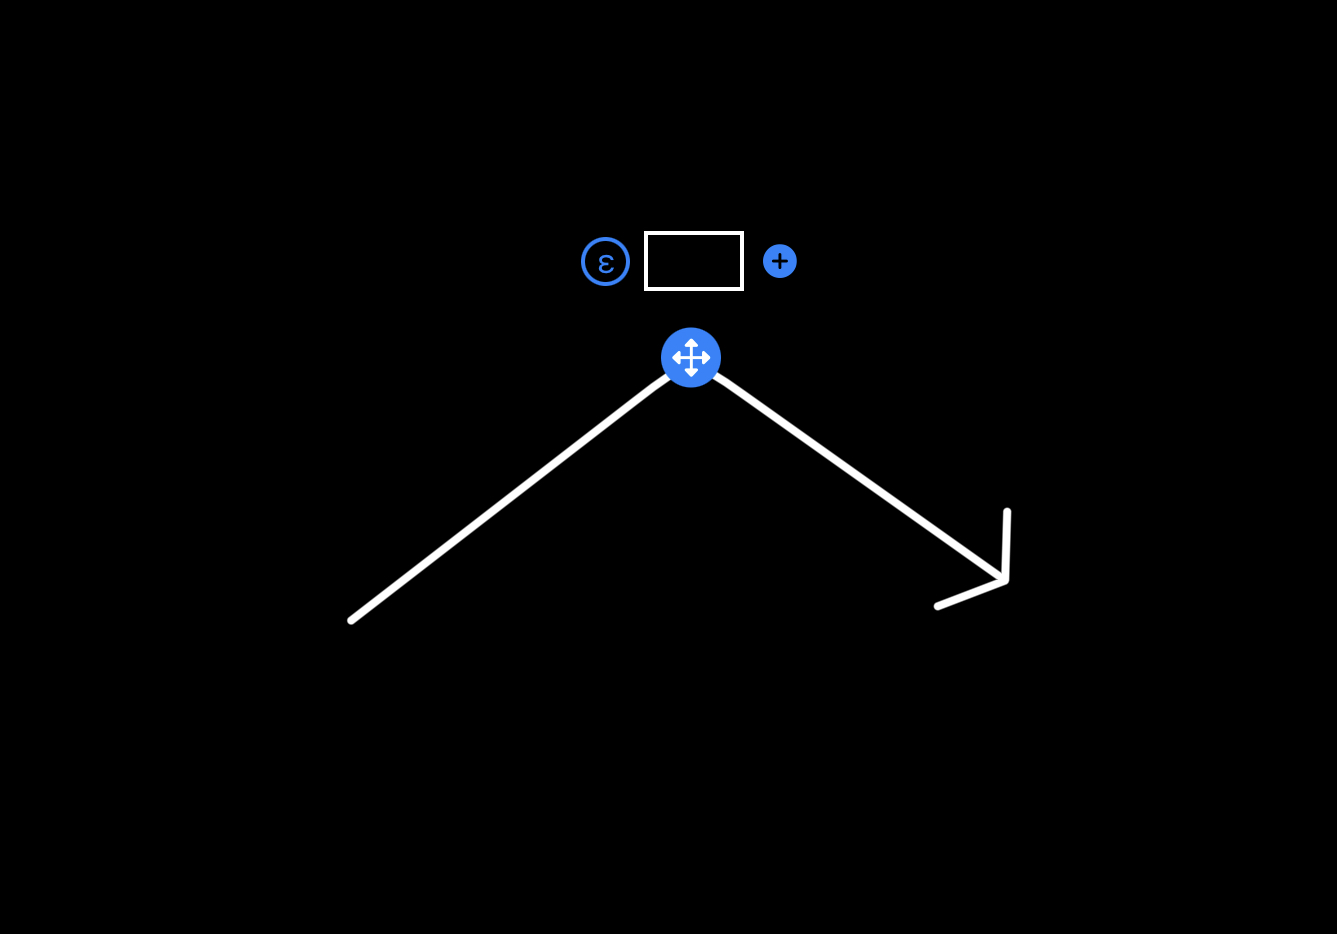
\includegraphics[width=0.4\textwidth]{spline-before}}
    \subfigure[]{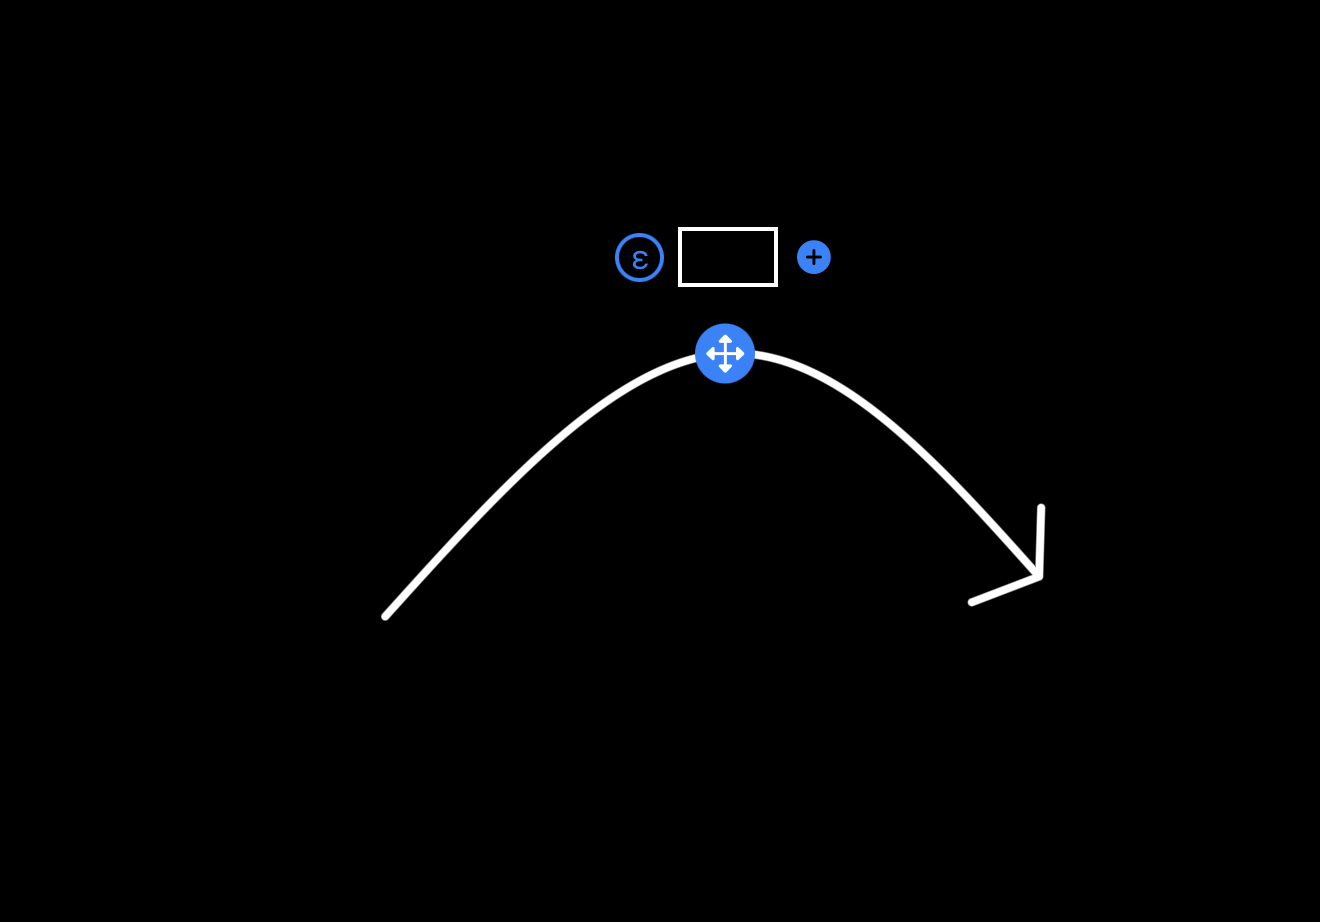
\includegraphics[width=0.4\textwidth]{spline-after}}
    \caption{Transition before using cubic spline (a) and after (b)}\label{spline}
\end{figure}

\begin{lstlisting}[caption={Creating spline points}, label=spline-code]
let points = [startPoint, flexPoint, tipPoint].compactMap { $0 }
let spline = Spline(
    values: points
)

let resolution = 100
let splinePoints: [CGPoint] = (
    0...(points.count - 1) * resolution
)
.map { offset in
    let argument = CGFloat(offset)/CGFloat(resolution)
    return spline.f(t: argument)
}
\end{lstlisting}

\subsection{Dragging States}

States are dragged as a whole and thus their shape is not changed during that process - the only variable in this process is a center of a given state. However, when a state has transitions connected to it, these transitions have to be changed as the state is dragged as well. There are three types of transitions that can be connected to a state - a transition that corresponds to an incoming or outcoming edge and a cycle. For cycles the app stores an angle between the single point that intersects with the state and a vector going from a center of the state and its topmost point. When the center is moved, the intersection point is recalculated with the angle that is stored in the app's state. For transitions other than cycles I take advantage of the \lstinline{flexPoint} and recompute \lstinline{startPoint} or \lstinline{endPoint} (depending on the transition) as the intersection point on the shortest path between the new center and the aforementioned \lstinline{flexPoint}. You can see that logic in \ref{compute-tippoint} for transitions that are the incoming edge.

\begin{lstlisting}[caption={Calculation of new \lstinline{tipPoint}}, label=compute-tippoint]
state.transitions
.filter { 
    $0.endState == automatonStateID 
    && $0.endState != $0.startState 
}
.forEach { transition in
    guard
        let flexPoint = transition.flexPoint,
        let endStateID = transition.endState,
        let endState = state.automatonStatesDict[endStateID]
    else { return }
    let vector = Vector(endState.center, flexPoint)
    state.transitionsDict[transition.id]?.tipPoint = vector.point(
        distance: endState.radius, 
        other: endState.center
    )
}
\end{lstlisting}
 
\section{DocumentGroup}

I have already outlined the intent to use a document based app approach to enable saving the editor's state into a file. Leveraging the benefits of using the Composable Architecture, I was able to save the whole state as JSON. To make that happen, I first had to conform \lstinline{EditorState} to a \lstinline{FileDocument} protocol. When a type conforms to this protocol it has to implement reading a file as well as saving it. The type must also declare on which extensions it will operate. For this app I have chosen the \lstinline{automaton} extension. This also ensures that the user cannot open a file that does not have that same extension (which would lead to undefined behaviour). To make an app a document based one, it is necessary to wrap a root view into a \lstinline{DocumentGroup} scene \cite{documentgroup}. 

\lstinline{DocumentGroup} is initialized with two parameters. \lstinline{newDocument} that describes what data should a new document contain - for the FA editor it is a new editor state - and then \lstinline{editor} closure that has the currently opened document as an input and it should return a view for editing the document. You can see how that is done for the automata editor here: \ref{documentgroup}. It should be noted that apart from initializing a new \lstinline{EditorStore} for a given document, as well as modifying the file when the state changes, it is also desirable to save stores for documents that have already been opened in the current application run. This is to ensure that a store is not reinitialized when a state changes which would cancel all currently running effects. The stores are saved into a dictionary \lstinline{stores} where each store is identified by the unique state's id. The UI for document based app is in figure \ref{document-based-interface}.

\begin{lstlisting}[caption={DocumentGroup scene}, label=documentgroup]
private final class DocumentStore {
    var stores: [UUID: EditorStore] = [:]
}

@main
struct AutomataEditorApp: App {
    private var documentStore = DocumentStore()
    
    var body: some Scene {
        DocumentGroup(
            newDocument: EditorState()
        ) { file -> EditorView in
            let store = documentStore.stores[file.document.id] 
            ?? EditorStore(
                initialState: file.document,
                reducer: editorReducer,
                environment: EditorEnvironment(...)
            )
            documentStore.stores[file.document.id] = store
            
            return EditorView(
                set: {
                    file.document = $0
                },
                store: store
            )
        }
    }
}
\end{lstlisting}

\begin{figure}
    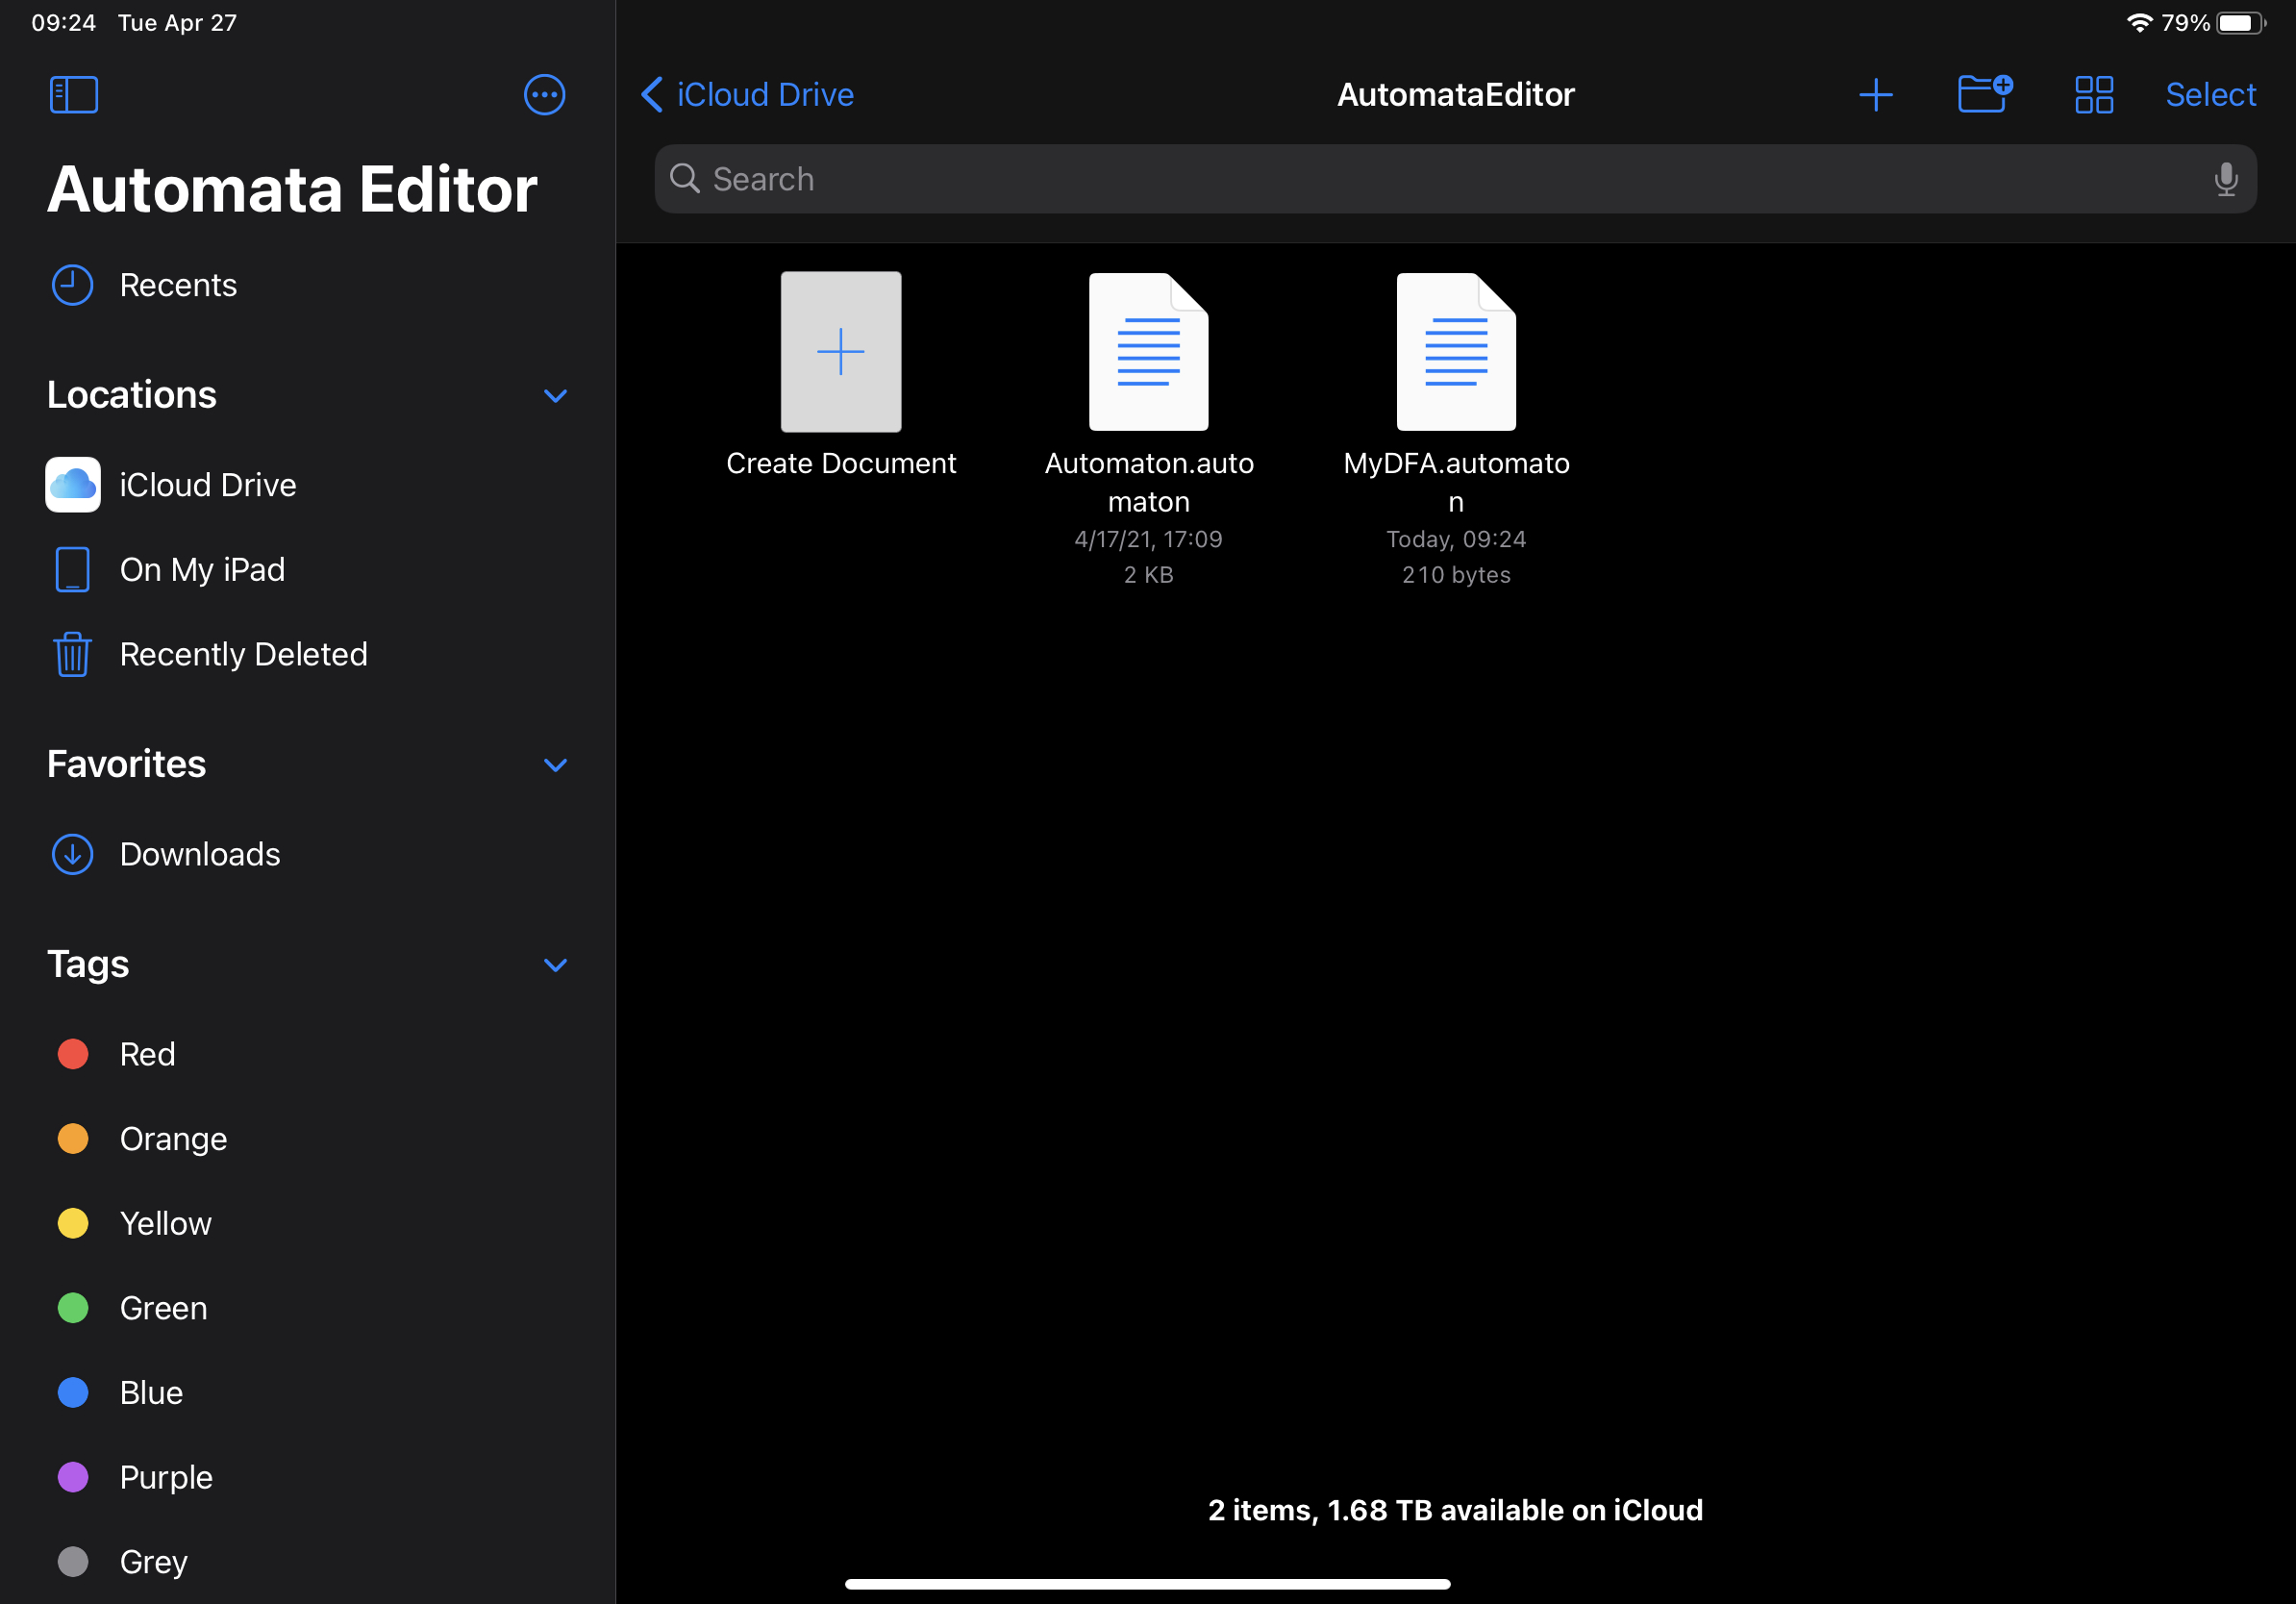
\includegraphics[width=\textwidth]{document-based}
    \caption{Document based app interface}\label{document-based-interface}
\end{figure}

\chapter{Testing}
\label{chap:testing}

Firstly, I will discuss how the app has been tested with automated tests. After that, I will go into how the usability testing has been conducted and what were its results and outcomes.

\section{Automated Testing}

Automated testing is an important part of a software project to ensure everything is working correctly and no regressions are made during the development. It also increases the confidence of doing refactoring. The Composable Architecture unit testing is built on top of the XCTest framework that is the bundled framework for testing Swift or Objective-C in Xcode. The goal of the testing in the Composable Architecture was to make tests more exhaustive, ergonomic and concise.

The main component for testing in the Composable Architecture is \lstinline{TestStore}. This component has a method called \lstinline{send} that takes as an input an action and a closure in which you describe how you expect the state to be modified. There is also a \lstinline{receive} method that asserts receival of a new action not triggered by the user, but rather returned from an effect. An example showcasing both \lstinline{send} and \lstinline{receive} methods can be seen in \ref{test-state} - there \lstinline{strokesChanged} action, that simulates a user drawing a stroke, is triggered first. When a stroke is drawn, it is sent to \lstinline{AutomataLibraryService} that returns \lstinline{Effect} with the recognized element (note that in the tests this component is mocked). When the new action \lstinline{automataShapeClassified} is received, I assert that it is added to the state.

It should be noted that the paradigm of this style of unit testing is focused on flows, rather than individual functions where the test asserts output for a given input - although individual functions can still be tested by sending a single action to the test store and asserting the state's changes. This is to make tests more concise and be closer to how the app will be used by the user. It does not mean, however, that the tests can be less reliable because still a single component is tested and all non-deterministic functionality should be in the store's environment, which is mocked during the testing. 

\begin{lstlisting}[caption={Testing creating of state}, label=test-state]
store.send(
    .strokesChanged(
        currentStrokes + [
            Stroke(controlPoints: [center])
        ]
    )
)
scheduler.advance()

store.receive(
    .automataShapeClassified(
        .success(
            .state(
                Stroke(
                    controlPoints: [center]
                )
            )
        )
    )
) {
    $0.automatonStatesDict[id] = AutomatonState(
        id: id,
        center: center,
        radius: radius
    )
}
\end{lstlisting}

\section{Usability Testing}

Usability testing does not have a strict definition but in general, it should refer to testing that evaluates a product or a system that is not automated. However, in the Handbook of Usability Testing the authors have narrowed this down to "a process that employs people as testing participants who are representative of the target audience to evaluate the degree to which a product meets specific usability criteria" \cite{handbook-usability-testing}. This book has also been used further in this section to define types of tests and their recommended techniques with which they should be conducted.

In the Handbook of Usability Testing the authors divide usability tests into four distinct categories: exploratory, assessment, validation, and comparison. Each test differs by its acceptance criteria and in which phase of the development it should be done. As the final product of this thesis is a prototype, the exploratory test is the most suitable one.

The primary focus of exploratory tests should be on the main functionalities of the app and to assess answers to questions such as how intuitive the design is, how valuable the product is for the user, which functionality will need to be documented via a tutorial or help, etc. This type of test is also different from the others in that it is expected that the moderator conducting the test will communicate with the user extensively - whereas the other tests should be possible to finish without the moderator stepping in.

\subsection{Test Plan}

Before tests could take place, it was necessary to create a test plan that was to be followed in the tests themselves. Test plans do not have to have the same components but the structure of the test plan for the Automata Editor app consists of:
\begin{itemize}
    \item Methodology
    \item Participant characteristics
    \item Introduction to the session
    \item Task list
    \item Final feedback
\end{itemize}

As outlined above, the test will be exploratory, implicating intensive interaction between the user and the mediator. Apart from that, it will be measured how long the individual tasks will take.

Before each test, the participants will be sent a questionnaire to assess their characteristics. It will include the following questions:
\begin{itemize}
    \item How familiar are you with finite automata? (rated 1-5 where 5 is "expert")
    \item Do you have prior experience with software for creating and editing finite automata?
    \item How familiar are you with using Apple Pencil in productivity applications - such as note-taking, drawing, creating diagrams, etc.? (rated 1-5 where 5 is "expert")
    \item Could you provide examples of software that you use with Apple Pencil?
\end{itemize}
These questions, although self-evaluated, should give a clearer picture of the user's previous experience with either finite automata or iPad usage.

During the introduction to the test, participants will be asked to think aloud, if they are comfortable with it. It is beneficial to know the thinking process as that can uncover more about the prototype. Then the user will be asked to do five tasks. These tasks are of two types:
\begin{itemize}
    \item Draw automaton based on a figure and test prescribed inputs.
    \item Draw automaton based on a formal definition of a language. The user has to come with inputs to test that it works properly.
\end{itemize}

The second type of tests (tasks D and E) is more complicated and therefore it will be done after the first one (tasks A-C). The tasks for each type will be randomized. Below you can find the individual tasks:

\begin{itemize}
    \item Task A:\\ 
    Create the automaton in \ref{task-a-automaton} and test the following inputs:
    \begin{itemize}
        \item AA
        \item BA
        \item B
        \item AAA
        \item ABA
        \item A
    \end{itemize}
    Then modify this automaton without clearing the canvas in such a way that it represents automaton in \ref{task-a-automaton-modified} and test the following inputs:
    \begin{itemize}
        \item ABBA
        \item ABAABA
        \item AAA
        \item BAB
        \item BBB
    \end{itemize}
    \item Task B:\\ 
    Create the automaton in \ref{task-b-automaton} and test the following inputs:
    \begin{itemize}
        \item DDE
        \item DEF
        \item DE
        \item EF
        \item EFE
        \item DDDDE
        \item DDDDF
    \end{itemize}
    \item Task C:\\ 
    Create the automaton in \ref{task-c-automaton} and test the following inputs:
    \begin{itemize}
        \item A
        \item BA
        \item AB
        \item ABB
    \end{itemize}
    \item Task D:\\
    Create automaton for the following language:\\
    \textit{L} = \{$(10)^{n}$: n $\in$ \textit{N}\}\\
    Simulate at least 4 inputs to test whether the automaton is behaving correctly.
    \item Task C:\\
    Create automaton for the following language:\\
    \textit{L} = \{w: w $\in$ $\{0,1\}^{*}$ $\wedge$ w starts with the string 011\}\\
    Simulate at least 4 inputs to test whether the automaton is behaving correctly.
\end{itemize}

\begin{figure}
    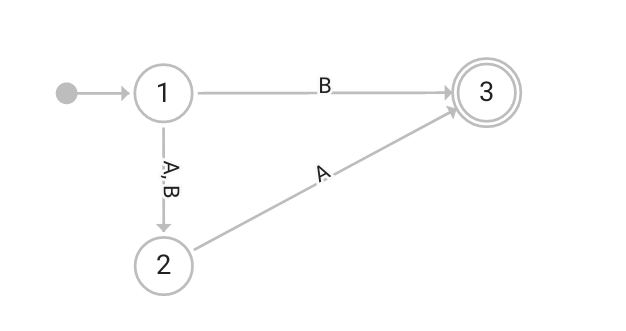
\includegraphics[width=\textwidth]{basic_automaton}
    \caption{Task A automaton}\label{task-a-automaton}
\end{figure}

\begin{figure}
    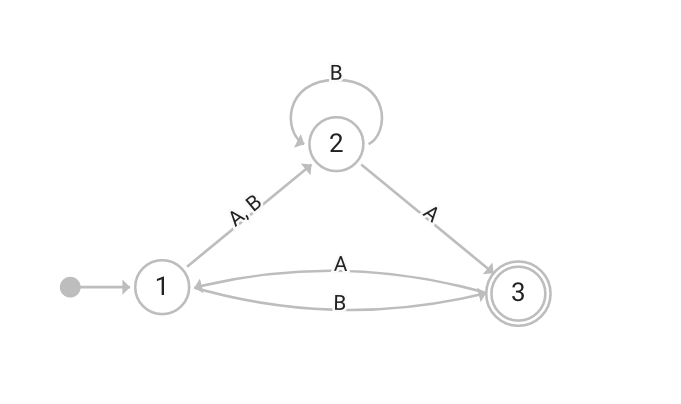
\includegraphics[width=\textwidth]{basic_automaton_2}
    \caption{Task A modified automaton}\label{task-a-automaton-modified}
\end{figure}

\begin{figure}
    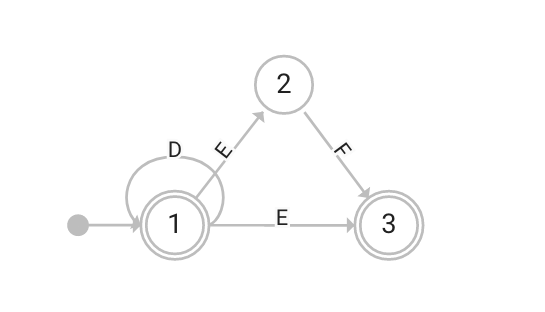
\includegraphics[width=\textwidth]{automaton_cycle}
    \caption{Task B automaton}\label{task-b-automaton}
\end{figure}

\begin{figure}
    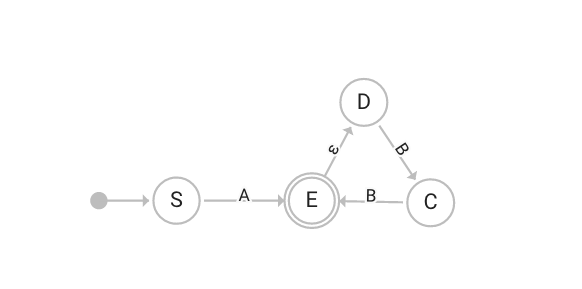
\includegraphics[width=\textwidth]{epsilon_automaton}
    \caption{Task C automaton}\label{task-c-automaton}
\end{figure}

\subsection{Test Results}

The tests have been done with a total of 8 participants. The results can be seen in \ref{test-results}. I have not included two questions in the table. One is whether the participant has prior experience with software for creating and editing finite automata - for which all answers have been "No". This indicates that most (in this case all) people have always used regular paper for sketching their automata. The second question not included is about examples of software that the participant has used with Apple Pencil: most of it were apps for making notes such as Notability or GoodNotes. From the time results the two fastest times are by people who rated themselves as FA "experts". In contrast with that is Apple Pencil familiarity having not a great impact on the time results. 

The following list summarizes what the participants have said they did not understand and where the design was not intuitive enough:
\begin{itemize}
    \item Plus button for adding multiple symbols to a single transition.
    \item When a state is deleted it's hard to reconnect it to transitions.
    \item Hard to understand output when it does not include any words.
    \item $\epsilon$ button was often not obvious.
    \item Clear was mistaken for back, deleting the whole automaton.
    \item Erasing button is not intuitive.
    \item It is hard to tell if the simulate button works if the output does not change.
\end{itemize}
Some of these points could be resolved by adding a quick tutorial and help that would introduce users into how the app should be used, rather than expecting users to figure it out on their own. The tutorial is also important since states and transitions are not added via a button and thus the users need to try and see how the app responds to their drawing. This can be a daunting first experience. 

The help feature, among others, was also mentioned by the participants as one of the following improvements:
\begin{itemize}
    \item Missing switch gesture for Apple Pencil.
    \item Back button to undo last change.
    \item Larger bottom control panel.
    \item Help or quick tutorial describing how the app should be used.
    \item Keyboard is too intrusive and often overlays text field currently being edited.
    \item It is not possible to make a state smaller.
    \item Make naming states not mandatory.
    \item Step-by-step simulation would help with visualization of how the FA works.
    \item Edit and presentation mode to hide and show buttons and text fields.
\end{itemize}
From this list, most of the items are small improvements and could be easily implemented into the app. I would like to expand on "step-by-step simulation". This feature would help with understanding better why the automaton rejected the input strings. It would also make it a great tool for learning and understanding how the automaton works. Implementing for DFAs should be possible as the automaton is always at one state only, making the visualization straightforward. However, for NFAs this is not the case. Therefore, the app could either offer to limit the automaton to a specific type or limit the visualization to only one possible path leading to rejection or acceptance. The usability testing has also uncovered a few bugs:
\begin{itemize}
    \item Input by keyboard is sometimes inadvertently triggered.
    \item Cycle is often mistaken for a state.
    \item Eraser sometimes does not work.
    \item It is not possible to make a final state a non-final one without deleting it.
    \item When a user taps on the screen in quick succession, transitions appear in the same place.
    \item Text field for transitions does not trim newlines.
\end{itemize}
All of these bugs are tracked in the \href{project's repository}{https://github.com/fortmarek/automata-editor}.

Apart from things that could be improved, at the end of each test I have asked the participants to say what they felt were good things about the app:
\begin{itemize}
    \item Eases learning of FAs.
    \item Simulating inputs is quick.
    \item Ability to save the FA in a file.
    \item Saving to a file is automatic.
    \item Making transitions with a simple line is fast.
    \item Recognizing elements is almost instant.
    \item Creating automata is quick once the user knows how to use the editor.
    \item Connecting elements works well.
    \item Interacting with elements is intuitive.
\end{itemize}
The positive comments show that the basic interactions with the elements work well and offer an enjoyable experience for the users. And apart from the enjoyable experience it makes creating the finite automata quick - which is important to convince people to use the app, rather than resorting to regular paper.

\begin{figure}
\begin{tabular}{||c|c|c|c||} 
    \hline
    Participant & Total time (mm:ss) & FA familiarity & Apple Pencil faimiliarity \\ [0.5ex] 
    \hline\hline
    A & 29:28 & 1 & 4\\ 
    \hline
    B & 10:30 & 5 & 1\\ 
    \hline
    C & 08:48 & 5 & 4\\ 
    \hline
    D & 15:26 & 3 & 1\\ 
    \hline
    E & 19:30 & 3 & 2\\ 
    \hline
    F & 25:12 & 3 & 4\\ 
    \hline
    E & 33:23 & 3 & 4\\ 
    \hline
    G & 25:58 & 5 & 3\\ 
    \hline
\end{tabular}
\caption{Usability testing results}\label{test-results}
\end{figure}

\chapter{Conclusion}

The primary goal of this thesis was to implement a prototype of an automata editor for iPad, built primarily for touch-based input and minimizing the need to use other UI controls such as buttons. The final prototype has focused on the Apple Pencil that offers a high level of precision while being easy to use. Most of the functionalities, like creating and editing FA elements, are done with the Apple Pencil, thus accomplishing the main goal. This was made possible by creating a custom ML model and using the CoreML framework to classify the drawn FA elements.

The chosen Composable Architecture has proved to be beneficial for the project as it allowed easy testing as well as a straightforward implementation of a document based app, which is an important feature for the users that was added on top of the originally outlined goals.

For simulating the input I have successfully leveraged the ALT library, proving that it can be integrated into a Swift-based project and used in iOS applications. This integration also opens many possible future directions this project can take as it can tap into the many functionalities the library offers, such as export of automatons in DOT and PNG format or FA algorithms like determinization and removal of $\epsilon$-transitions.

In the conducted usability testing, which has uncovered some minor issues with the prototype, it has also been suggested by some of the participants to add a step-by-step simulation of the input, so the users can better visualize how the particular FA operates. This functionality would also have to be implemented in the ALT library by e.g. returning a trace of the individual steps taken by the FA. Another feature that has been raised during the testing was adding support for a pushdown automaton.

One of the main motivations of this project was to help students learning FAs. To accomplish this, the prototype needs some smaller improvements but it is planned to publish it on the App Store before the winter semester of the 2021/2022 school year, so it can be suggested to students taking the BI-AAG course at FIT CTU in Prague.

The feedback I have been given in the usability testing has made it clear that the prototype, even in the current state, would be beneficial for students learning the FAs, therefore, I deem the prototype to be successful.
